% -----------------------------------------------------------------------------
% Chapters 3 and 4: perturbations of isolated singularities and experiments.
%
% This file compiles on its own (chapters 1 and 2 are empty stubs). To use it
% in the thesis, copy the two \chapter blocks into the main file, after the
% numerical isosurface extraction chapter, together with
%   * \usepackage{booktabs}            (tables)
%   * the \thesisimage macro below     (image placeholders)
%   * the entries of chapters3_4_references.bib in bibliography.bib.
%
% Images: put the files listed in FIGURES.md into pictures/ch3/ and
% pictures/ch4/. Until a file exists, a framed placeholder with its name and
% content description is printed instead.
%
% Labels from chapter 1 used here: sec:singularities, def:regular-singular,
% sec:blowup (please add \label{sec:blowup} to the section "Blowup and
% Resolution of Singularities"), and def:edge-interp from chapter 2.
% -----------------------------------------------------------------------------
% !!! ALWAYS COMPILE THIS FILE !!!

\documentclass[12pt, a4paper, oneside]{book}

%%%%%%%%%%%%%%%%%%%%%%%%%%%%%%%%%%%%%%%%%%%%%%%%%%%%%%%%
% 														%
%  					 Basic formatting 					%
% 														%
%%%%%%%%%%%%%%%%%%%%%%%%%%%%%%%%%%%%%%%%%%%%%%%%%%%%%%%%

% Page margins
\usepackage[top=2.5cm, bottom=2.5cm, right=2cm, left=3.5cm]{geometry}

% Line height
\linespread{1.5}

% !!! optional !!!  no hyphenation
\tolerance=100000000
\hyphenpenalty 10000000
\exhyphenpenalty 10000000

% Insert pdf
\usepackage{pdfpages}

% Charset
\usepackage[utf8]{inputenc}
\usepackage[T1]{fontenc}

% Common packages (math fonts, floats etc.)
\usepackage{amsthm}
\usepackage{amsmath}
\usepackage{amsfonts}
\usepackage{float}
\usepackage{array}
\usepackage{pdflscape}
\usepackage{calc}
\usepackage[linesnumbered, ruled]{algorithm2e}
\usepackage{caption}
\usepackage{tikz}
\usepackage{graphicx}
\usepackage{comment}
\usepackage{subcaption}
\usepackage{booktabs}

%%%%%%%%%%%%%%%%%%%%%%%%%%%%%%%%%%%%%%%%%%%%%%%%%%%%%%%%
% 													 %
%  					Optional formatting 				 %
% 													 %
%%%%%%%%%%%%%%%%%%%%%%%%%%%%%%%%%%%%%%%%%%%%%%%%%%%%%%%%

% Theorems
\theoremstyle{plain}
\newtheorem{theorem}{Theorem}[chapter]
\newtheorem{lemma}[theorem]{Lemma}
\newtheorem{proposition}[theorem]{Proposition}
\newtheorem{corollary}[theorem]{Corollary}

% Definitions and examples
\theoremstyle{definition}
\newtheorem{definition}[theorem]{Definition}
\newtheorem{example}[theorem]{Example}

% Remarks
\theoremstyle{remark}
\newtheorem{remark}[theorem]{Remark}

\usepackage{caption}
\captionsetup[figure]{labelfont=bf}
\captionsetup[table]{labelfont=bf}

% !!! optional !!! package for drawing graphs
\usepackage{pgfplots}
\pgfplotsset{width=14cm, height=10cm, compat=1.9}

% !!! optional !!! package for displaying a code
\usepackage{listings}
\definecolor{dkgreen}{rgb}{0,0.6,0}
\definecolor{gray}{rgb}{0.8,0.8,0.7}
\definecolor{myteal}{rgb}{0.17,0.57,0.69}
\definecolor{whitish}{rgb}{0.99, 0.99, 0.98}
\definecolor{mauve}{rgb}{0.58,0,0.82}

\lstset{frame=tb,
  backgroundcolor=\color{whitish},
  language=C++,
  aboveskip=3mm,
  belowskip=0mm,
  showstringspaces=false,
  columns=flexible,
  basicstyle={\footnotesize\ttfamily},
  numbers=none,
  numberstyle=\tiny\color{gray},
  keywordstyle=\color{blue},
  commentstyle=\color{dkgreen},
  stringstyle=\color{mauve},
  breaklines=true,
  breakatwhitespace=true,
  tabsize=3,
  emph={int,char,double,float,unsigned,void,bool,MyMesh, VertexIter, VertexVertexCCWIter, std, vector, VertexHandle, vec, AngleOf, max, min} ,
  emphstyle={\color{teal}},
  captionpos=b,
  frame=single,
  rulecolor=\color{gray}
}
\renewcommand{\lstlistingname}{Code excerpt}
\captionsetup[lstlisting]{labelfont=bf}
\renewcommand\lstlistlistingname{Source codes}

% Image or, while the file does not exist yet, a framed placeholder.
%   #1 file, #2 width, #3 placeholder height, #4 what the image must show
\newcommand{\thesisimage}[4]{%
  \IfFileExists{#1}{\includegraphics[width=#2]{#1}}{%
    \fbox{\parbox[c][#3][c]{#2}{\centering\footnotesize
      \textbf{Image placeholder}\\[2pt]\texttt{\detokenize{#1}}\\[4pt]#4}}}}

%%%%%%%%%%%%%%%%%%%%%%%%%%%%%%%%%%%%%%%%%%%%%%%%%%%%%%%%
% 														%
%  			 Information about the author 				%
% 														%
%%%%%%%%%%%%%%%%%%%%%%%%%%%%%%%%%%%%%%%%%%%%%%%%%%%%%%%%

\def\skola{Comenius University in Bratislava}
\def\fakulta{Faculty of Mathematics, Physics and Informatics}
\def\autor{Lucia Držková}

\begin{document}

%\pagenumbering{roman}

\newpage
\title{Singularity-aware isosurface extraction}
\newpage
\chapter{Implicit Surfaces and Singularities}
\chapter{Numerical Isosurface Extraction}

% =============================================================================
\chapter{Perturbations of Isolated Singularities}
\label{ch:perturbation-theory}
% =============================================================================

Section~\ref{sec:singularities} showed that the regular structure of an implicit
surface breaks down at points where the gradient vanishes, and the previous
chapter showed that this is exactly where voxel-based extraction becomes
unreliable. A natural way to study such a point is to embed the singular surface
into a family of nearby surfaces and observe what happens as the family
approaches it. This chapter develops that point of view for one-parameter
perturbations
\[
H_k = F + kG ,
\]
in which the surface $\{F=0\}$ has an isolated singular point and $G$ is a
fixed polynomial. The chapter is organised around three questions.
\begin{enumerate}
    \item[(Q1)] In which sense, and how fast, does the perturbed surface
          $\{H_k=0\}$ approach the singular surface $\{F=0\}$ as $k\to0$?
    \item[(Q2)] What happens to the singular point itself, and are new singular
          points created? If so, how many, where, and of which local type?
    \item[(Q3)] Which of these effects can a uniform voxel grid resolve?
\end{enumerate}
The answers depend on two properties of $G$: the order of its first nonzero
Taylor term at the singular point, which fixes the characteristic length scale
of the deformation, and its direction, that is, its coefficients, which decide
whether singular points survive, disappear, or are created. Chapter~\ref{ch:experimental-results}
tests every statement of this chapter numerically.

% -----------------------------------------------------------------------------
\section{One-Parameter Families of Implicit Surfaces}
\label{sec:families}

Let $F,G:\mathbb{R}^3\to\mathbb{R}$ be polynomials and let
\begin{equation}
\label{eq:perturbed-family}
H_k(p)=F(p)+kG(p),\qquad
S_k=\{p\in\mathbb{R}^3: H_k(p)=0\},\qquad k\in\mathbb{R}.
\end{equation}
The unperturbed surface $S_0=\{F=0\}$ is recovered at $k=0$. We assume that
$S_0$ has an isolated singular point $p_0$, and after a translation we take
$p_0=0$. All statements are local: they concern the intersection of $S_k$ with
a closed ball $\overline{B}_R=\{p:\|p\|\le R\}$ around the origin, for $|k|$ small.
The behaviour for $k\to0^-$ and for $k\to0^+$ is studied separately, since
the two one-sided limits can be different.

\begin{definition}[Singular point of a perturbed surface]
\label{def:singular-perturbed}
A point $q\in\mathbb{R}^3$ is a \emph{singular point of $S_k$} if
\begin{equation}
\label{eq:singularity-system}
H_k(q)=0
\qquad\text{and}\qquad
\nabla H_k(q)=0 .
\end{equation}
A point satisfying only $\nabla H_k(q)=0$ is a \emph{stationary point} of
$H_k$.
\end{definition}

% Both conditions in~\eqref{eq:singularity-system} are essential, in accordance with Definition~\ref{def:regular-singular}. 
A stationary point with
$H_k(q)\neq0$ does not lie on $S_k$ and has no influence on the regularity of
the surface. The distinction matters throughout this chapter: a perturbation
typically creates several stationary points near the origin, and only those on
the zero level are singular points of the surface.

% -----------------------------------------------------------------------------
\section{The Reference Singularity}
\label{sec:reference-singularity}

The experiments in Chapter~\ref{ch:experimental-results} use the two cubic
polynomials
\begin{equation}
\label{eq:F-sigma}
F_\sigma(x,y,z)=x^3+y^3+\sigma z^3,\qquad \sigma\in\{+1,-1\},
\end{equation}
written $F_+$ and $F_-$. Their gradients $(3x^2,3y^2,3\sigma z^2)$ vanish only
at the origin, which therefore is the unique singular point of
$S_0=\{F_\sigma=0\}$ (Figure~\ref{fig:reference-cones}).

\begin{figure}[!h]
    \centering
    \begin{subfigure}{0.47\textwidth}
        \centering
        %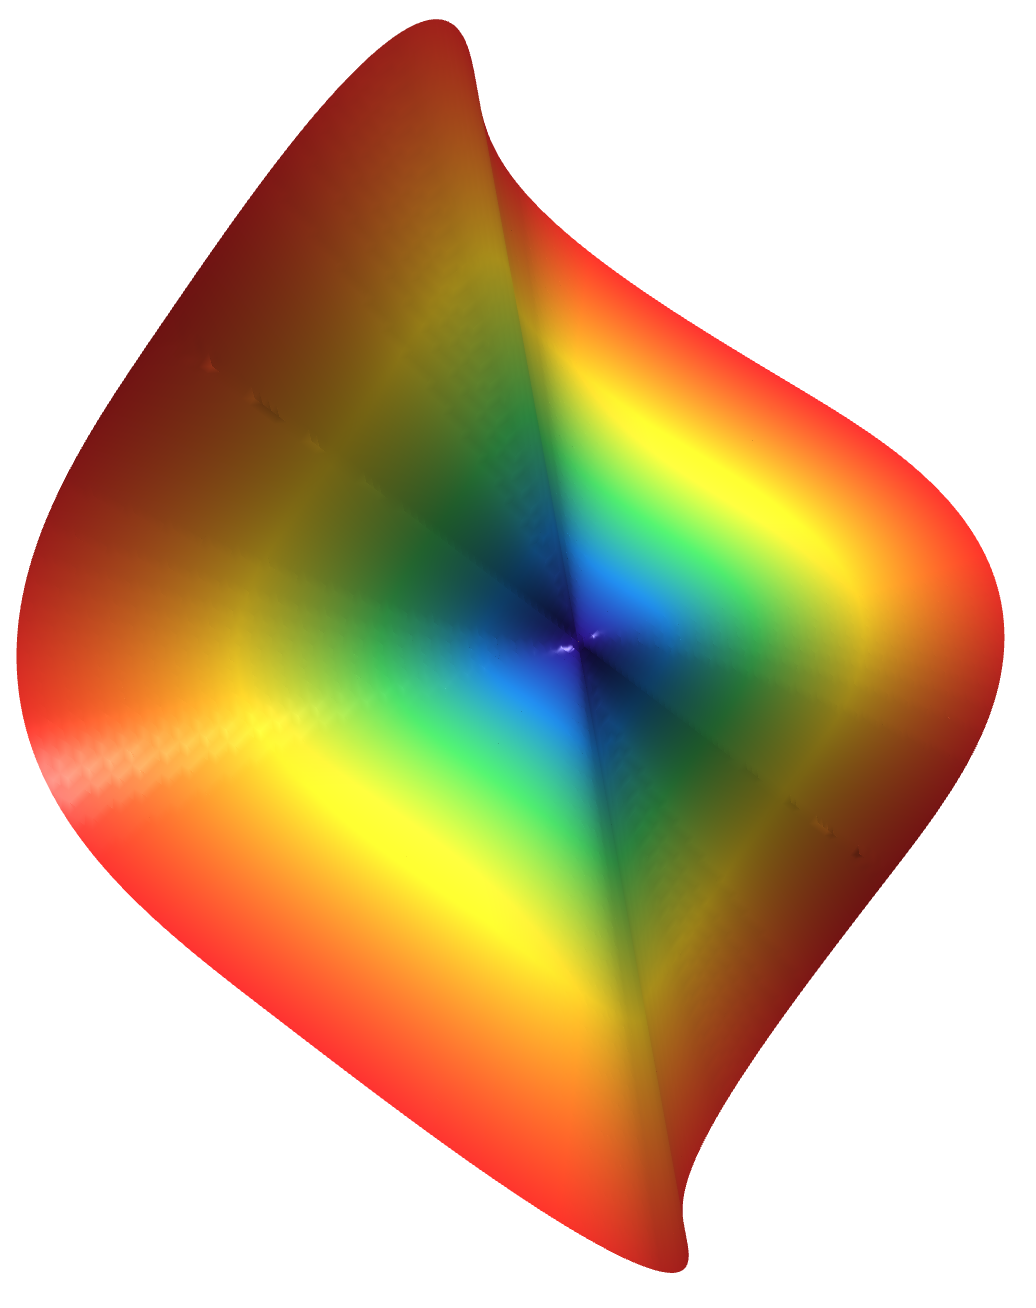
\includegraphics[width=0.7\linewidth]{pictures/ch3/cone_Fplus.png}
        \thesisimage{pictures/ch3/cone_Fplus.png}{\textwidth}{5cm}{$S_0$ for $F_+=x^3+y^3+z^3$, 3D view coloured by $\|\nabla F\|$}
        \caption{$F_+=x^3+y^3+z^3$}
    \end{subfigure}
    \hfill
    \begin{subfigure}{0.47\textwidth}
        \centering
        %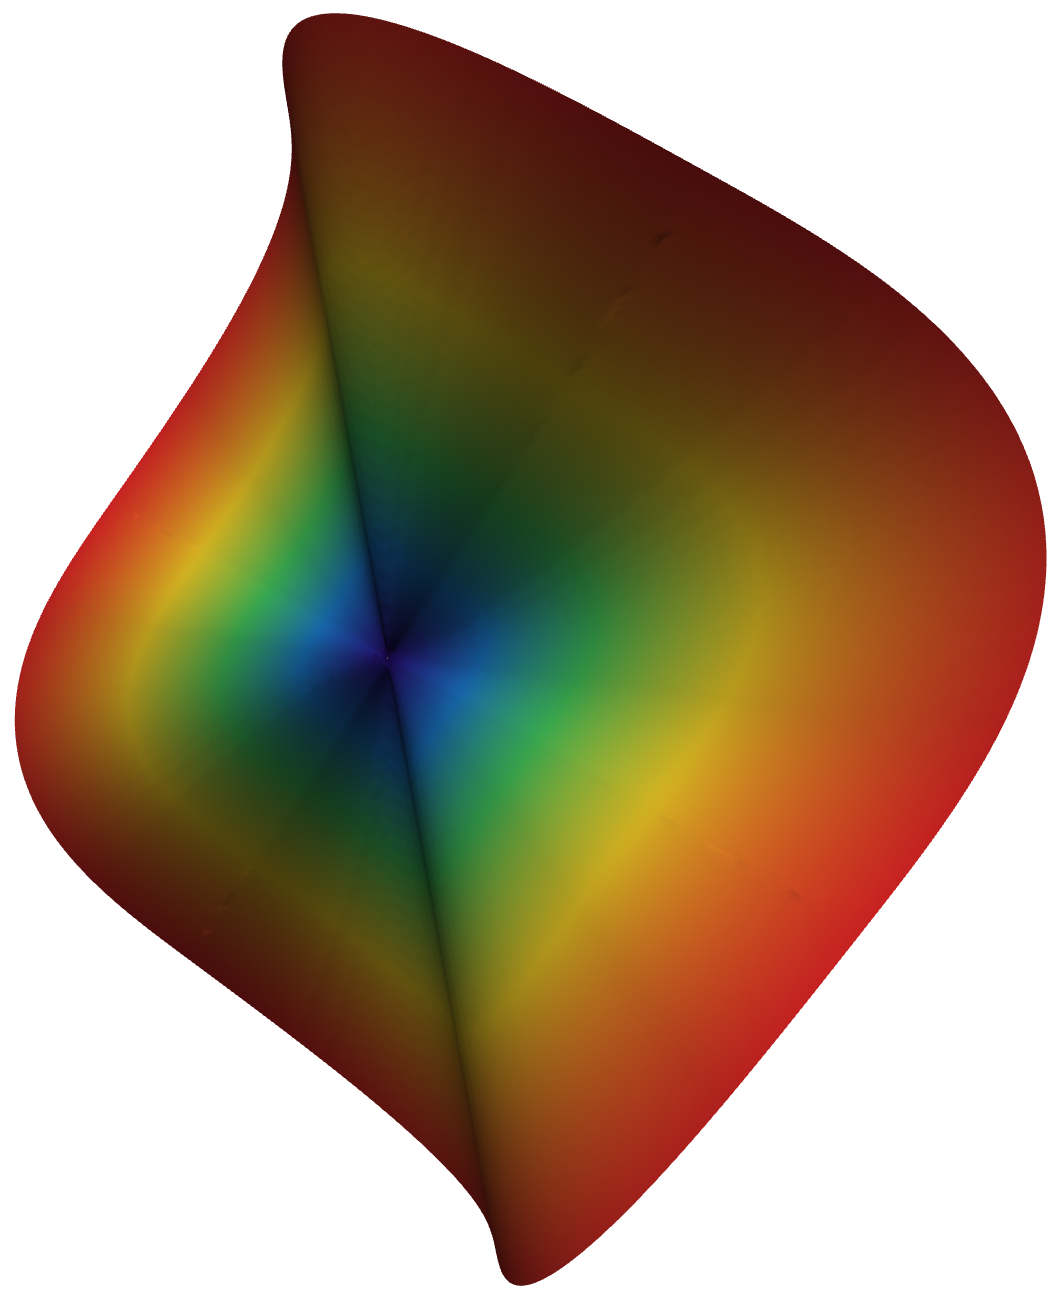
\includegraphics[width=0.7\linewidth]{pictures/ch3/cone_Fminus.png}
        \thesisimage{pictures/ch3/cone_Fminus.png}{\textwidth}{5cm}{$S_0$ for $F_-=x^3+y^3-z^3$, same view and colour scale}
        \caption{$F_-=x^3+y^3-z^3$}
    \end{subfigure}
    \caption[Reference cones]{The two reference surfaces. Both are cones with
    their apex, the only singular point, at the origin. Colour encodes
    $\|\nabla F\|$, which vanishes at the apex.}
    \label{fig:reference-cones}
\end{figure}

\paragraph{Homogeneity and the cone structure.}
Both polynomials are homogeneous of degree three, $F_\sigma(tp)=t^3F_\sigma(p)$.
Hence $p\in S_0$ implies $tp\in S_0$ for every $t\in\mathbb{R}$, so $S_0$ is a
cone with apex at the origin, made of the lines through the origin and the
points of the curve $S_0\cap\{\|p\|=1\}$. Moreover, $\nabla F_\sigma(p)\neq0$
for all $p\neq0$: every point of the cone except the apex is regular. The
reference singularity is therefore isolated, although its Hessian matrix
vanishes and its first nonzero Taylor term has order three. A vanishing Hessian
is a sign of a degenerate singularity, not of a non-isolated one.

The cone contains real lines. Since
$x^3+y^3=(x+y)(x^2-xy+y^2)$, the line $\{x+y=0,\ z=0\}$ lies on
$\{F_+=0\}$, and the same holds for $\{x+z=0,\ y=0\}$ and $\{y+z=0,\ x=0\}$.
These lines pass exactly through nodes of a symmetric voxel grid, which is
relevant for the numerical treatment in Chapter~\ref{ch:experimental-results}.

\paragraph{Reflection.}
The two reference polynomials are related by the reflection
$\rho(x,y,z)=(x,y,-z)$: $F_-=F_+\circ\rho$. Consequently
\begin{equation}
\label{eq:reflection}
F_-+kG=(F_++k\,G\circ\rho)\circ\rho ,
\end{equation}
so the family $F_-+kG$ is the mirror image of the family $F_++k\,(G\circ\rho)$.
For example, $F_-+k(x+z)$ behaves like $F_++k(x-z)$. Every result for $F_+$
transfers to $F_-$ by replacing $z$ with $-z$ in the perturbation; a fixed
perturbation such as $x+z$, however, is a different perturbation for the two
reference surfaces.

\paragraph{Local type and Milnor number.}
The algebraic complexity of an isolated singularity is measured by its
\emph{Milnor number}
\begin{equation}
\label{eq:milnor-number}
\mu(F,0)=\dim_{\mathbb{R}}\,
\mathbb{R}[x,y,z]_{(x,y,z)}\big/\big(\tfrac{\partial F}{\partial x},
\tfrac{\partial F}{\partial y},\tfrac{\partial F}{\partial z}\big),
\end{equation}
the dimension of the local algebra modulo the gradient ideal
\cite{milnor1968singular,greuel2007introduction}. For $F_\sigma$ the gradient
ideal is generated by $x^2$, $y^2$ and $z^2$, so the quotient has the basis
\begin{equation}
\label{eq:milnor-basis}
1,\ x,\ y,\ z,\ xy,\ xz,\ yz,\ xyz,
\end{equation}
and $\mu(F_\sigma,0)=8$. In the classification of singularities, a cone over a
smooth plane cubic curve is the \emph{simple elliptic singularity}
$\tilde{E}_6$ \cite{arnold2012singularities}. It is the most degenerate
isolated singularity a cubic surface can have; the remaining possibilities,
ordered by increasing Milnor number, are $A_1,\dots,A_5$, $D_4$, $D_5$ and
$E_6$ \cite{bruce1979classification}. The Milnor number will reappear in
Section~\ref{sec:perturbation-vector} as an upper bound on the number of singular
points that a perturbation can create.

% -----------------------------------------------------------------------------
\section{The Original Point Under Perturbation}
\label{sec:taylor-perturbation}

At the origin $F(0)=0$ and $\nabla F(0)=0$, hence
\begin{equation}
\label{eq:origin-value-gradient}
H_k(0)=kG(0),\qquad
\nabla H_k(0)=k\nabla G(0),\qquad
\operatorname{Hess}H_k(0)=\operatorname{Hess}F(0)+k\operatorname{Hess}G(0).
\end{equation}
The first two identities decide the fate of the origin for every $k\neq0$:
\begin{itemize}
    \item if $G(0)\neq0$, the origin \emph{leaves} the surface;
    \item if $G(0)=0$ and $\nabla G(0)\neq0$, the origin \emph{stays on} $S_k$
          as a \emph{regular} point, and its gradient grows linearly,
          $\|\nabla H_k(0)\|=|k|\,\|\nabla G(0)\|$;
    \item if $G(0)=0$ and $\nabla G(0)=0$, the origin \emph{remains singular}
          for every $k$.
\end{itemize}
In the third case the Hessian identity in~\eqref{eq:origin-value-gradient}
describes how the singularity changes. For $F_\sigma$ the Hessian vanishes, so
$\operatorname{Hess}H_k(0)=k\operatorname{Hess}G(0)$. If this matrix is
nonsingular, the origin becomes an ordinary double point ($A_1$, a quadratic
cone); if it has rank one, the singularity is degenerate in two directions. For
$G=x^2$ the leading terms at the origin become $kx^2+y^3+\sigma z^3$, which is
the normal form of a $D_4$ singularity \cite{arnold2012singularities}: the
singular point persists, but it is simpler ($\mu=4$) than the original
$\tilde{E}_6$ ($\mu=8$). None of these tests excludes additional singular
points away from the origin; those still have to be found from the full
system~\eqref{eq:singularity-system}.

\begin{definition}[Order of the perturbation]
\label{def:order}
Write the Taylor expansion of $G$ at the origin as
$G=G_0+G_1+G_2+\cdots$, where $G_j$ is homogeneous of degree $j$. The
\emph{order} of $G$ is the smallest $m$ with $G_m\neq0$.
\end{definition}

The order is a local quantity and need not equal the total degree. The
polynomial $G=x^2+x$ has degree two but order $m=1$, because its linear term
dominates near the origin. The three cases above correspond to $m=0$, $m=1$ and
$m\ge2$.

% -----------------------------------------------------------------------------
\section{Notions of Convergence}
\label{sec:convergence-notions}

The statement ``$S_k$ converges to the singular surface'' admits several
precise meanings, which can have different answers for the same family.

\begin{definition}[Local Hausdorff distance]
\label{def:local-hausdorff}
For closed sets $A,B\subset\mathbb{R}^3$ and $R>0$, put $A_R=A\cap\overline{B}_R$,
$B_R=B\cap\overline{B}_R$ and
\[
d_R(A,B)=\max\Big\{\sup_{a\in A_R}\operatorname{dist}(a,B),\ \sup_{b\in B_R}\operatorname{dist}(b,A)\Big\},
\]
the Hausdorff distance of the two sets restricted to the ball
\cite{rockafellar1998variational}. We write $d_R(k)=d_R(S_k,S_0)$.
\end{definition}

\begin{definition}[Convergence notions]
\label{def:convergence-types}
Let $\sigma\in\{-,+\}$ denote one side of $k=0$.
\begin{enumerate}
    \item \textbf{Set convergence.} $S_k\to S_0$ near the origin as
          $k\to0^\sigma$ if every point of $S_0\cap B_R$ is a limit of points
          of $S_k$, and every limit of points of $S_k\cap \overline{B}_R$ lies
          in $S_0$ (Painlevé--Kuratowski convergence
          \cite{rockafellar1998variational}).
    \item \textbf{Convergence with rate $\alpha$.} $d_R(k)=\Theta(|k|^\alpha)$
          as $k\to0^\sigma$, that is,
          $c|k|^\alpha\le d_R(k)\le C|k|^\alpha$ for small $|k|$. We call the
          convergence \emph{Lipschitz} if $\alpha=1$ and \emph{Hölder} if
          $0<\alpha<1$.
    \item \textbf{Convergence of singular points.} Singular points $q(k)$ of
          $S_k$ converge to the origin with rate $\gamma$ if
          $\|q(k)\|=\Theta(|k|^\gamma)$.
    \item \textbf{Gradient behaviour.} The size of $\nabla H_k$ at the origin,
          given by~\eqref{eq:origin-value-gradient}, and the minimum of
          $\|\nabla H_k\|$ on $S_k$ near the origin, which measures how close
          $S_k$ is to being singular.
\end{enumerate}
\end{definition}

These notions measure different things. If $G(0)=0$, the distance from the
origin to $S_k$ is zero for every $k$, although the surface does change; set
convergence holds while the normals of $S_k$ near the origin never converge,
because $S_0$ has no tangent plane there; and new singular points can converge
to the origin while the origin itself becomes regular. The two parts of set
convergence behave very differently, as the next two propositions show.

\begin{proposition}[Limits stay on the singular surface]
\label{prop:upper-limit}
If $q_k\in S_k\cap\overline{B}_R$ and $q_k\to q$ along a sequence $k\to0$, then
$q\in S_0$. This holds for every polynomial $G$.
\end{proposition}

\begin{proof}
$G$ is bounded on $\overline{B}_R$, so $F(q_k)=-kG(q_k)\to0$, and $F(q)=0$ by
continuity.
\end{proof}

\begin{proposition}[Sign-change criterion]
\label{prop:sign-change}
Let $p\in S_0$ be a point such that $F$ takes both signs in every
neighbourhood of $p$. Then for every $\varepsilon>0$ there is $\delta>0$ such
that $S_k$ meets the ball $B_\varepsilon(p)$ whenever $0<|k|<\delta$.
\end{proposition}

\begin{proof}
Choose $a,b\in B_\varepsilon(p)$ with $F(a)<0<F(b)$, and let
$M=\max|G|$ on the segment $[a,b]$. For
$|k|<\delta=\min\{|F(a)|,|F(b)|\}/M$, the polynomial $H_k$ is negative at $a$
and positive at $b$, so it vanishes on the segment by the intermediate value
theorem.
\end{proof}

For $F_\sigma$ the hypothesis holds at every point of $S_0$: at regular points
because the gradient is nonzero, and at the origin because $F_\sigma$ is odd,
$F_\sigma(-p)=-F_\sigma(p)$. Together with Proposition~\ref{prop:upper-limit},
$S_k$ converges to $S_0$ in the sense of sets from \emph{both} sides of $k=0$,
for \emph{every} perturbation $G$. Set convergence can only fail where $F$ does
not change sign. For $F=x^2+y^2+z^2$ and $G=1$, the surface $S_k$ is empty for
$k>0$ and a sphere of radius $\sqrt{|k|}$ for $k<0$, so the convergence is
one-sided.

A lower bound on the rate follows from homogeneity.

\begin{proposition}[Universal bound for the reference cones]
\label{prop:lojasiewicz}
There is $c>0$ with $|F_\sigma(p)|\ge c\,\operatorname{dist}(p,S_0)^3$ for all
$p\in\mathbb{R}^3$. Consequently, for every polynomial $G$,
\[
\sup_{q\in S_k\cap\overline{B}_R}\operatorname{dist}(q,S_0)
\le\Big(\frac{|k|\max_{\overline{B}_R}|G|}{c}\Big)^{1/3}.
\]
\end{proposition}

\begin{proof}[Sketch]
On the unit sphere, $|F_\sigma(\omega)|/\operatorname{dist}(\omega,S_0)$ is
bounded below near $S_0$ because $\nabla F_\sigma\neq0$ there, and it is
positive and continuous elsewhere; since $\operatorname{dist}(\omega,S_0)\le2$,
this gives $|F_\sigma(\omega)|\ge c\operatorname{dist}(\omega,S_0)^3$. For
$p=r\omega$ both sides scale by $r^3$, because $S_0$ is a cone. The second
statement follows from $|F_\sigma(q)|=|k||G(q)|$ on $S_k$.
\end{proof}

This is a special case of the Łojasiewicz inequality
\cite{lojasiewicz1959division}. It bounds one half of the Hausdorff distance:
no point of $S_k$ is farther than $O(|k|^{1/3})$ from $S_0$, whatever $G$ is.
The finer behaviour is described by a scaling argument.

% -----------------------------------------------------------------------------
\section{Scaling and the Model Surface}
\label{sec:scaling-law}

Let $F$ be homogeneous of degree three with $\nabla F(p)\neq0$ for $p\neq0$, as
is the case for $F_\sigma$, and let $G$ have order $m<3$. Substituting
$p=\lambda u$ with $\lambda>0$ gives
\[
H_k(\lambda u)=\lambda^3F(u)+k\lambda^mG_m(u)+k\,O(\lambda^{m+1}).
\]
The two leading terms are of the same size when $|k|\lambda^m=\lambda^3$, that is,
for the \emph{characteristic scale}
\begin{equation}
\label{eq:scaling-law}
\lambda(k)=|k|^{1/(3-m)} .
\end{equation}
Dividing by $\lambda^3$ and writing $\sigma=\operatorname{sign}k$,
\begin{equation}
\label{eq:rescaled}
\frac{H_k(\lambda u)}{\lambda^3}=F(u)+\sigma G_m(u)+O(\lambda),
\end{equation}
so in the coordinates $u=p/\lambda$ the family converges to the fixed
\emph{model surface}
\begin{equation}
\label{eq:model-surface}
M_\sigma=\{u\in\mathbb{R}^3:\ F(u)+\sigma G_m(u)=0\}.
\end{equation}
Geometrically, $S_k$ near the origin is a copy of $M_\sigma$ shrunk by the factor
$\lambda(k)$, while away from the origin it is a small displacement of the cone
$S_0$. Figure~\ref{fig:inner-outer} sketches the two regions.

\begin{figure}[!h]
\centering
\begin{tikzpicture}[scale=1.6]
    % outer ball
    \draw[dashed, gray] (0,0) circle (1.9);
    \node[gray] at (1.55,1.55) {$\overline{B}_R$};
    % inner region
    \draw[dashed, red!70!black] (0,0) circle (0.55);
    \node[red!70!black, font=\small] at (0.3,-0.75) {$\|p\|\sim\lambda(k)$};
    % the cone S_0 (two lines)
    \draw[thick, black] (-1.8,-1.8) -- (1.8,1.8);
    \draw[thick, black] (-1.8,1.8) -- (1.8,-1.8);
    \node[font=\small] at (-1.55,1.25) {$S_0$};
    % perturbed surface: two hyperbola branches
    \draw[thick, teal, domain=-1.25:1.25, samples=60, smooth]
        plot ({0.32*cosh(\x)}, {0.32*sinh(\x)});
    \draw[thick, teal, domain=-1.25:1.25, samples=60, smooth]
        plot ({-0.32*cosh(\x)}, {0.32*sinh(\x)});
    \node[teal, font=\small] at (1.45,0.55) {$S_k$};
    \fill (0,0) circle (0.03);
    \node[font=\small] at (0.12,0.15) {$0$};
\end{tikzpicture}
\caption[Inner and outer region]{Schematic cross-section. Far from the origin
(outer region) $S_k$ is a displacement of the cone $S_0$ of size $O(|k|)$.
Inside a ball of radius proportional to $\lambda(k)$ (inner region) it is a
scaled copy of the model surface $M_\sigma$, which here has opened the
singularity.}
\label{fig:inner-outer}
\end{figure}

The rescaling $p=\lambda u$ is the weighted blowup of
Section~\ref{sec:blowup} applied to the point $(p,k)=(0,0)$ of the four
dimensional space of positions and parameters, with weight one for the spatial
variables and weight $3-m$ for $k$. The model surface is the surface seen in
the chart $\bar k=\pm1$. In this sense the blowup is not only a tool for
dynamical systems; here it resolves the singular limit $k\to0$ of a family of
implicit surfaces.

\begin{proposition}[Scaling]
\label{prop:scaling}
Let $F$ be homogeneous of degree three with $\nabla F\neq0$ away from the
origin, let $G$ have order $m<3$, and fix the side $\sigma$. Then, as
$k\to0^\sigma$:
\begin{enumerate}
    \item the rescaled surfaces $\lambda(k)^{-1}S_k$ converge to $M_\sigma$ on
          compact sets, and smoothly near every regular point of $M_\sigma$;
    \item every nondegenerate singular point $u^\ast$ of $M_\sigma$ gives a
          singular point $q(k)=\lambda(k)u^\ast+o(\lambda)$ of $S_k$ of the same
          type, and $S_k$ has no other singular points at distance
          $O(\lambda)$ from the origin; in particular $S_k$ is regular near the
          origin if $M_\sigma$ is regular;
    \item $d_R(k)=O(\lambda(k))$, and $d_R(k)=\Theta(\lambda(k))$ whenever
          $M_\sigma$ differs from the cone $S_0$, so that the rate of
          convergence is $\alpha=1/(3-m)$.
\end{enumerate}
\end{proposition}

\begin{proof}[Sketch]
By~\eqref{eq:rescaled}, the rescaled polynomials converge with all derivatives
on compact sets. At regular points of $M_\sigma$ the implicit function theorem
gives (1); applied to the gradient system it gives (2). Because
$\nabla F\neq0$ away from the origin, the rescaled surfaces stay close to the
cone outside a large ball in the $u$-coordinates, which gives the uniform
bound in (3); the lower bound comes from a point where $M_\sigma$ and the cone
are at positive distance.
\end{proof}

The proposition is a special case of the theory of deformations of
quasi-homogeneous singularities
\cite{arnold2012singularities,greuel2007introduction}; the sketch indicates the
mechanism rather than a complete proof. Table~\ref{tab:scaling} lists the
consequences for the reference cones.

\begin{table}[!h]
\centering
\small
\begin{tabular}{c c c l}
\toprule
Order $m$ & Balance & Scale $\lambda(k)$ & Behaviour at the origin \\
\midrule
$0$ & $r^3\sim|k|$       & $|k|^{1/3}$ & leaves the surface \\
$1$ & $r^3\sim|k|\,r$    & $|k|^{1/2}$ & stays on $S_k$, becomes regular \\
$2$ & $r^3\sim|k|\,r^2$  & $|k|$       & stays singular, type simplifies \\
$3$ & same degree        & ---         & stays singular, cone changes shape \\
\bottomrule
\end{tabular}
\caption[Scaling regimes]{Scaling regimes for a homogeneous cubic $F$ with
$\nabla F\neq0$ away from the origin. For $m=3$ no shrinking scale exists:
$F+kG_3$ is again a cubic cone, and $d_R(k)$ is proportional to $|k|$ on a
fixed ball.}
\label{tab:scaling}
\end{table}

\begin{example}[Constant perturbation]
For $G=1$ the model surface $M_\sigma=\{F(u)=-\sigma\}$ does not contain the
origin and is smooth, because $\nabla F$ vanishes only at the origin. Hence
$S_k$ is regular near the origin and lies at distance
$\lambda(k)\operatorname{dist}(0,M_\sigma)$ from it. For $F_\sigma$ this
distance is computed exactly in Section~\ref{sec:constant-perturbation}.
\end{example}

\begin{example}[Coordinate perturbation]
For $F_+$ and $G=x$ the model surface is $u^3+v^3+w^3+\sigma u=0$. Its
stationary points satisfy $3u^2=-\sigma$ and $v=w=0$, and there the value is
$u(u^2+\sigma)=\tfrac{2\sigma}{3}u\neq0$. The model surface is smooth, so $S_k$
is regular near the origin for both signs of $k$, and the rate of convergence
is $\alpha=1/2$.
\end{example}

\begin{remark}[Non-homogeneous singularities]
\label{rem:weighted}
If the leading part of $F$ is only \emph{weighted} homogeneous, for example
$x^2+y^2+z^3$ (an $A_2$ singularity, with weights $\tfrac12,\tfrac12,\tfrac13$
satisfying $F(t^{1/2}x,t^{1/2}y,t^{1/3}z)=t\,F(x,y,z)$), the same argument uses
an anisotropic rescaling. If $G$ has weighted order $d_w(G)<1$, the scale is
$\lambda=|k|^{1/(1-d_w(G))}$, the deformation along axis $i$ is of size
$\lambda^{w_i}$, and the rate lies between
$w_{\min}/(1-d_w(G))$ and $w_{\max}/(1-d_w(G))$. For the homogeneous cubic all
weights equal $\tfrac13$ and $d_w(G)=m/3$, which gives back
$\alpha=1/(3-m)$.
\end{remark}

% -----------------------------------------------------------------------------
\section{The Perturbation as a Vector}
\label{sec:perturbation-vector}

The perturbation $G$ can be regarded as a vector in three complementary ways.

\paragraph{The gradient of a linear perturbation.}
For $G=ax+by+cz$ the gradient $\nabla G=(a,b,c)$ is constant, so the
perturbation adds the constant vector $k(a,b,c)$ to the gradient field of $F$.
At the origin it becomes the normal of $S_k$, by~\eqref{eq:origin-value-gradient}.
The direction of this vector decides where real stationary points can appear,
as Section~\ref{sec:linear-perturbation} shows.

\paragraph{A direction in the space of polynomials.}
Polynomials of degree at most three form a vector space of dimension twenty,
with the coefficients of the twenty monomials $x^iy^jz^l$, $i+j+l\le3$, as
coordinates. The reference polynomial $F$ is a point of this space, and the
family $F+kG$ is the straight line through $F$ in the direction of the vector
$G$. Polynomials whose zero set is singular form a hypersurface of this space,
the \emph{discriminant}. Whether $S_k$ is regular for small $k\neq0$ depends
on how the line leaves the discriminant at $F$: a line that crosses it gives
regular surfaces on both sides, while a line that stays inside it keeps a
singular point for all $k$.

\paragraph{Essential and inessential directions.}
Not every direction changes the singularity. A perturbation that equals, to
first order, a change of coordinates only moves or distorts the surface.

\begin{lemma}[First-order coordinate changes]
\label{lem:trivial-directions}
If $G=\sum_i a_i\,\partial F/\partial x_i$ with polynomial coefficients $a_i$,
then $H_k(p)=F\big(p+k\,a(p)\big)+O(k^2)$, where $a=(a_1,a_2,a_3)$.
\end{lemma}

\begin{proof}
This is the first-order Taylor expansion of $F(p+ka(p))$ in $k$.
\end{proof}

For $F_\sigma$, whose gradient ideal is generated by $x^2,y^2,z^2$, two cases
are exact rather than first-order:
\begin{align}
\label{eq:translation}
x^3+kx^2&=\Big(x+\frac k3\Big)^3-\frac{k^2}{3}\,x-\frac{k^3}{27},\\
\label{eq:stretch}
x^3+kx^3&=\big(\sqrt[3]{1+k}\;x\big)^3 .
\end{align}
The perturbation $x^2$ is therefore, up to terms of order $k^2$, a
\emph{translation} of the cone by $k/3$ along the $x$-axis, and $x^3$ is
exactly a \emph{linear stretch} of the cone along the $x$-axis. Only the
directions that remain after removing such coordinate changes, the classes of
$G$ modulo the gradient ideal, are \emph{essential} for the singularity. They
form the vector space with basis~\eqref{eq:milnor-basis}, which is the
parameter space of the versal deformation of the singularity
\cite{arnold2012singularities,greuel2007introduction}. Writing $G$ in this
basis is the most informative way of treating it as a vector: constant and
linear terms open the singularity, the mixed terms $xy,xz,yz$ change its type,
and $xyz$ moves the cone within the family of cubic cones.

\paragraph{Conservation of the Milnor number.}
For small $k$, the Milnor numbers of all \emph{complex} stationary points of
$H_k$ near the origin add up to $\mu(F,0)$
\cite{milnor1968singular,greuel2007introduction}. For the reference cones the
total is always eight, and a perturbation redistributes it, as
Table~\ref{tab:milnor-conservation} shows. Two consequences are useful. First,
a perturbation of $F_\sigma$ creates at most eight singular points near the
origin. Second, whether a stationary point is visible at all depends on the
sign of $k$: stationary points that are real for one sign are complex for the
other.

\begin{table}[!h]
\centering
\small
\begin{tabular}{l l c c}
\toprule
$G$ & stationary points of $H_k$ near $0$ & $\sum\mu$ & on $S_k$ \\
\midrule
$1$           & the origin ($\tilde E_6$)                            & $8$ & none \\
$x$           & $(\pm\sqrt{-k/3},0,0)$, type $D_4$ ($\mu=4$ each)    & $8$ & none \\
$x+y$         & $(\pm\sqrt{-k/3},\pm\sqrt{-k/3},0)$, type $A_2$ ($\mu=2$ each) & $8$ & two \\
$x+y+z$       & eight points, type $A_1$                             & $8$ & none \\
$x^2$         & $0$ and $(-2k/3,0,0)$, type $D_4$                    & $8$ & the origin \\
$x^2+y^2-z^2$ & eight points, type $A_1$                             & $8$ & three \\
\bottomrule
\end{tabular}
\caption[Conservation of the Milnor number]{Redistribution of the Milnor
number $\mu(F_+,0)=8$. For the linear perturbations the listed points are real
for $k<0$ and complex for $k>0$; for the quadratic ones they are real for both
signs. The
last column counts the points on the zero level, which are the singular points
of $S_k$.}
\label{tab:milnor-conservation}
\end{table}

% -----------------------------------------------------------------------------
\section{Linear Perturbations: An Exact Criterion}
\label{sec:linear-perturbation}

For linear perturbations of the reference cones, all singular points can be
found in closed form. We state the result for a general diagonal cubic, which
contains both $F_+$ and $F_-$.

\begin{proposition}[Singular points under linear perturbation]
\label{prop:linear}
Let $F=a_1x_1^3+a_2x_2^3+a_3x_3^3$ with $a_i\neq0$, let
$G=c_1x_1+c_2x_2+c_3x_3\neq0$, and let $k\neq0$.
\begin{enumerate}
    \item The stationary points of $H_k=F+kG$ are the points with
          $3a_ix_i^2=-kc_i$ for $i=1,2,3$; they are real if and only if
          $kc_ia_i\le0$ for every $i$.
    \item At every stationary point $q$,
          \begin{equation}
          \label{eq:level-at-stationary}
          H_k(q)=\frac{2k}{3}\,G(q).
          \end{equation}
    \item Consequently, $S_k$ has a singular point if and only if the
          stationary points are real and there are signs
          $\varepsilon_i\in\{-1,+1\}$ (for the indices with $c_i\neq0$) with
          \begin{equation}
          \label{eq:balance}
          \sum_{i:\,c_i\neq0}\varepsilon_i\,c_i\,\Big|\frac{c_i}{a_i}\Big|^{1/2}=0 .
          \end{equation}
          Each such sign choice gives one singular point
          $q_i=\varepsilon_i\sqrt{|kc_i/(3a_i)|}$, at distance
          \begin{equation}
          \label{eq:singular-distance}
          \|q\|=\sqrt{\frac{|k|}{3}}\,\Big(\sum_i\Big|\frac{c_i}{a_i}\Big|\Big)^{1/2}
          \end{equation}
          from the origin. Singular points therefore converge to the origin
          with rate $\gamma=1/2$.
    \item At such a point $\operatorname{Hess}H_k(q)=\operatorname{diag}(6a_iq_i)$.
          The singular point is an ordinary double point ($A_1$) if all $c_i$
          are nonzero, and a cusp ($A_2$) if exactly one $c_i$ vanishes.
\end{enumerate}
\end{proposition}

\begin{proof}
(1) is the gradient equation. For (2), at a stationary point
$a_ix_i^3=x_i\cdot a_ix_i^2=-kc_ix_i/3$, so $F(q)=-\tfrac k3G(q)$ and
$H_k(q)=\tfrac{2k}{3}G(q)$. For (3), a stationary point is singular exactly
when $G(q)=0$; inserting $q_i$ gives $\sqrt{|k|/3}$ times the left-hand side
of~\eqref{eq:balance}. A single nonzero $c_i$ cannot satisfy~\eqref{eq:balance}.
For (4), the Hessian is diagonal with entries $6a_iq_i$, which vanish exactly
when $c_i=0$; one vanishing entry with a nonzero cubic term $a_ix_i^3$ in that
direction gives the normal form of $A_2$.
\end{proof}

\begin{example}
\label{ex:linear-cases}
For $F_+$, real stationary points require all nonzero $c_i$ to have the sign
opposite to $k$. The balance condition~\eqref{eq:balance} becomes
$\sum\varepsilon_i|c_i|^{3/2}=0$.
\begin{itemize}
    \item $G=x$: $\pm1\neq0$, no singular points.
    \item $G=x+y$: $1-1=0$, two cusps $(\pm\sqrt{-k/3},\mp\sqrt{-k/3},0)$ for $k<0$,
          at distance $\sqrt{2|k|/3}$; the same for $x+z$ and $y+z$.
    \item $G=x+y+z$: $\pm1\pm1\pm1\neq0$, stationary points for $k<0$ but no
          singular points.
    \item $G=2x+4y+6z$: $2^{3/2}\pm4^{3/2}\pm6^{3/2}\neq0$, no singular points;
          similarly $9x+y+3z$, $x+2y+3z$ and $2x+4y+z$.
    \item $G=x+y+2^{2/3}z$: $1+1-(2^{2/3})^{3/2}=0$, two ordinary double points
          with all three coordinates nonzero, for $k<0$.
\end{itemize}
For $F_-$ the coefficient $a_3=-1$ reverses the sign condition on $c_3$. Thus
$x+z$, $y+z$, $x+y+z$ and $2x+4y+6z$ have no real stationary points at all,
while $x+y$ still produces two cusps and $x+y-2^{2/3}z$ two ordinary double
points. This is the reflection~\eqref{eq:reflection} at work.
\end{example}

The proposition answers questions (Q1) and (Q2) completely for linear
perturbations: the order $m=1$ fixes the scale $|k|^{1/2}$, while the
coefficient vector decides, through a sign condition and the balance
condition~\eqref{eq:balance}, whether singular points exist, how many there are
and of which type.

% -----------------------------------------------------------------------------
\section{Consequences for Voxel-Based Extraction}
\label{sec:voxel-consequences}

A uniform grid with spacing $h$ cannot represent features smaller than a few
grid cells. The scale $\lambda(k)$ of Section~\ref{sec:scaling-law} therefore
splits every family into two numerical regimes.
\begin{itemize}
    \item If $\lambda(k)\gg h$, the inner region is resolved: the grid sees the
          opened singularity, new singular points can be located, and $d_R(k)$
          can be measured.
    \item If $\lambda(k)\lesssim h$, the extracted mesh of $S_k$ is
          numerically indistinguishable from that of $S_0$. The grid then shows
          a singular-looking surface even though $S_k$ is regular.
\end{itemize}
For the reference cones the deformation is of size $|k|^{1/3}$ for $m=0$ and
$|k|^{1/2}$ for $m=1$. For $m=2$, by~\eqref{eq:translation}, it is about
$|k|/3$, and for the stretch~\eqref{eq:stretch} it is at most $|k|R/3$ on the
ball of radius $R$. With $|k|=0.01$ and $h\approx0.007$, the first two are many
grid cells wide, the third is below one cell, and the last is below a tenth of
a cell. A distance measured on a mesh is moreover only meaningful between the
mesh accuracy, of the order of $h$, and the size $R$ of the region in which it
is measured. Chapter~\ref{ch:experimental-results} therefore fits convergence
rates only to values in the window $h/2\le d_R(k)\le0.6R$, and chooses the
range of $k$ separately for each order.

For singularity-aware extraction this gives a concrete design rule. A surface
with a singular point is represented faithfully near that point only if the
grid resolves the scales at which the surface changes. For a perturbed surface
this means $h\ll\lambda(k)$; for the singular surface itself it means that the
neighbourhood of the singular point has to be refined adaptively, or treated
analytically, since no finite uniform spacing resolves a structure that exists
at every scale.


% =============================================================================
\chapter{Experimental Results}
\label{ch:experimental-results}
% =============================================================================

This chapter tests the theory of Chapter~\ref{ch:perturbation-theory} on the
two reference cones $F_\pm=x^3+y^3\pm z^3$ and twenty-five perturbations $G$
covering the orders zero to three. Each claim about singular points is first
derived from the exact equations~\eqref{eq:singularity-system} and then compared
with the numerical results; the convergence rates are measured on extracted
meshes and compared with the scaling prediction.

% -----------------------------------------------------------------------------
\section{Experimental Setup}
\label{sec:setup}

\paragraph{Families.}
For each reference polynomial $F_+$ and $F_-$ the perturbations in
Table~\ref{tab:perturbations} were tested, grouped by their order $m$ at the
origin.

\begin{table}[!h]
\centering
\small
\begin{tabular}{c l}
\toprule
Order $m$ & Perturbations $G$ \\
\midrule
$0$ & $1$ \\
$1$ & $x,\ y,\ z,\ x+y,\ x+z,\ y+z,\ x+y+z,\ 2x+4y+6z,\ 9x+y+3z,\ x+2y+3z,\ 2x+4y+z$, \\
    & $x+y\pm2^{2/3}z$ (balanced, $+$ for $F_+$ and $-$ for $F_-$),\ $x^2+x,\ x^2+y,\ x^2+z$ \\
$2$ & $x^2,\ y^2,\ z^2,\ x^2+y^2+z^2,\ x^2+y^2-z^2$ \\
$3$ & $x^3,\ y^3,\ z^3$, and $G=F$ \\
\bottomrule
\end{tabular}
\caption[Tested perturbations]{The tested perturbations, by order at the
origin. The same list was used for $F_+$ and $F_-$.}
\label{tab:perturbations}
\end{table}

\paragraph{Numerical settings.}
The surfaces were extracted on the domain $[-0.4,0.4]^3$ with $48$, $96$ and
$110$ cells per axis, giving grid spacings $h=0.016667$, $0.008333$ and
$0.007273$. Every family was sampled at $25$ uniformly spaced parameters
$k\in[-0.01,0.01]$ (twelve negative, zero, twelve positive). For rate fits, every
family was in addition sampled at nine logarithmically spaced values of $|k|$ on
each side at resolution $110$, with $|k|\in[10^{-4},10^{-2}]$ for orders zero and
one and $|k|\in[3\cdot10^{-3},0.3]$ for orders two and three, where the
deformation is otherwise below the grid spacing
(Section~\ref{sec:voxel-consequences}). All local measurements use the ball of
radius $R=0.18$ around the origin.

\paragraph{Extraction.}
The surfaces were extracted with the Marching Cubes method described in the
previous chapters, using linear edge interpolation
(Definition~\ref{def:edge-interp}). Grid nodes at which $F$
vanishes, exactly or up to rounding errors, are moved to the positive side by a
small deterministic amount when several of their edges would otherwise produce
the same intersection point. Vertex normals and gradient magnitudes are
evaluated exactly by automatic differentiation of $H_k$ at the vertices.

\paragraph{Measurements.}
For every value of $k$ the following quantities were recorded.
\begin{itemize}
    \item The distance from the origin to the mesh, computed exactly as the
          minimum point-to-triangle distance.
    \item The local Hausdorff distance $d_R(k)$, estimated by sampling points on
          the triangles of each mesh inside the ball and measuring their exact
          distance to the triangles of the other mesh. This is a sampled
          approximation of Definition~\ref{def:local-hausdorff}, not its exact
          value; an average (root mean square) distance was recorded as well.
          A margin of two grid cells is excluded at the boundary of the ball,
          to avoid artefacts of the clipping.
    \item The minimum of $\|\nabla H_k\|$ over mesh vertices in the ball.
    \item Stationary points of $H_k$ in the ball, found by a damped Newton
          method started at the origin and at 26 surrounding points, with points closer than $10^{-3}h$
          merged, and classified as singular when $H_k$ also vanishes within a
          tolerance relative to the magnitude of its terms. The local type is
          read from the rank of the Hessian.
\end{itemize}
A convergence rate is obtained by a least-squares fit of
$\log d=\log C+\alpha\log|k|$, separately for $k<0$ and $k>0$, using only values
inside the resolvable window $h/2\le d\le0.6R$ and requiring at least three
values spanning a factor of two in $|k|$.

\paragraph{Reproducibility.}
All runs were produced by the program \texttt{isosurface\_chapter4\_experiments}
of the accompanying software, which writes one folder of CSV files per family
and resolution, and the classification tables summarised in
Section~\ref{sec:classification-summary}. The interactive viewer performs the
same analysis with the \emph{Classify convergence} action.

% -----------------------------------------------------------------------------
\section{The Reference Surfaces}
\label{sec:reference-results}

At $k=0$ the stationary-point search finds only the origin, with
$F_\pm=0$, a vanishing gradient and a vanishing Hessian, in agreement with
Section~\ref{sec:reference-singularity}. The real lines of the cones pass
through grid nodes: at resolution $110$ the grid contains $331$ nodes at which
$F_+$ vanishes exactly. The tie-break described above handles them; the meshes
of the reference cones contain no degenerate triangles.

% -----------------------------------------------------------------------------
\section{Constant Perturbation}
\label{sec:constant-perturbation}

For $G=1$ the origin leaves the surface and the gradient of $H_k$ vanishes only
at the origin, so $S_k$ has no singular points for $k\neq0$. The distance from
the origin to $S_k$ can be computed exactly.

\begin{proposition}
\label{prop:constant-distance}
For $F_\pm$ and $k\neq0$, $\operatorname{dist}(0,S_k)=|k|^{1/3}$.
\end{proposition}

\begin{proof}
Minimise $\|p\|^2$ subject to $x^3+y^3\pm z^3=-k$. The Lagrange condition
$2x_i=3\nu a_ix_i^2$ (with $a_i=\pm1$) forces each coordinate to be either zero
or equal to $2/(3\nu a_i)$, so the nonzero coordinates have equal absolute
value $s$. With $j$ nonzero coordinates of the appropriate signs, the
constraint gives $js^3=|k|$ and the distance $\sqrt j\,s=j^{1/6}|k|^{1/3}$. The
minimum is attained for $j=1$, at a point on a coordinate axis.
\end{proof}

The surface therefore converges to the cone from both sides with rate
$\alpha=1/3$ and constant $C=1$, and $S_k$ leaves the ball of radius $0.18$
when $|k|>0.18^3\approx0.0058$. Only the seven smallest values of $|k|$ on each
side are therefore usable; the larger ones correctly report no local surface.
Table~\ref{tab:constant-fit} compares the measured distances with the exact
result.

\begin{table}[!h]
\centering
\small
\begin{tabular}{c c c c c}
\toprule
Cells per axis & Fitted $\alpha$ & Fitted $C$ & $R^2$ & Largest relative error \\
\midrule
$48$  & $0.33592$ & $1.01279$ & $0.9999582$ & $7.5\cdot10^{-3}$ \\
$96$  & $0.33386$ & $1.00240$ & $0.9999990$ & $1.6\cdot10^{-3}$ \\
$110$ & $0.33343$ & $1.00006$ & $0.9999993$ & $7.8\cdot10^{-4}$ \\
\midrule
exact & $1/3$ & $1$ & & \\
\bottomrule
\end{tabular}
\caption[Constant perturbation: distance fits]{Fits of
$\operatorname{dist}(0,S_k)=C|k|^\alpha$ for $G=1$, using the fourteen values
of $k$ for which the surface meets the ball. The results for $F_+$ and $F_-$
are identical, as expected from the reflection symmetry. The last column is
the largest relative deviation from $|k|^{1/3}$.}
\label{tab:constant-fit}
\end{table}

The fitted values approach the exact ones under refinement, and the largest
relative error decreases by a factor of about five from $48$ to $96$ cells,
consistent with the second-order accuracy of linear edge interpolation.
Figure~\ref{fig:constant-plot} shows the measured distances. This is the most
direct validation of the extraction and measurement pipeline, because the
reference value is known exactly. The local Hausdorff distance follows the same
law: its fitted exponent is $0.34$ on both sides.

\begin{figure}[!h]
\centering
\begin{tikzpicture}
\begin{axis}[
    width=0.62\textwidth, height=0.42\textwidth,
    xmode=log, ymode=log,
    xlabel={$|k|$}, ylabel={$\operatorname{dist}(0,S_k)$},
    legend pos=north west, legend cell align=left,
    grid=major, grid style={gray!25}]
\addplot[only marks, mark=*, mark size=1.6pt, blue] coordinates {
(0.000833333,0.0940696) (0.00166667,0.11847) (0.0025,0.135633) (0.00333333,0.149292)
(0.00416667,0.160879) (0.005,0.17092) (0.00583333,0.179958)};
\addlegendentry{measured, 110 cells}
\addplot[only marks, mark=o, mark size=2.2pt, red] coordinates {
(0.000833333,0.0933953) (0.00166667,0.118339) (0.0025,0.135481) (0.00333333,0.149306)
(0.00416667,0.160514) (0.005,0.170693) (0.00583333,0.179757)};
\addlegendentry{measured, 48 cells}
\addplot[black, domain=0.0007:0.007, samples=10] {x^(1/3)};
\addlegendentry{exact $|k|^{1/3}$}
\end{axis}
\end{tikzpicture}
\caption[Constant perturbation: distance]{Distance from the origin to the
extracted mesh of $F_++k=0$ for $k>0$, on logarithmic axes. The exact law
$|k|^{1/3}$ is a straight line of slope $1/3$.}
\label{fig:constant-plot}
\end{figure}

\begin{figure}[!h]
    \centering
    \begin{subfigure}{0.31\textwidth}
        \centering
        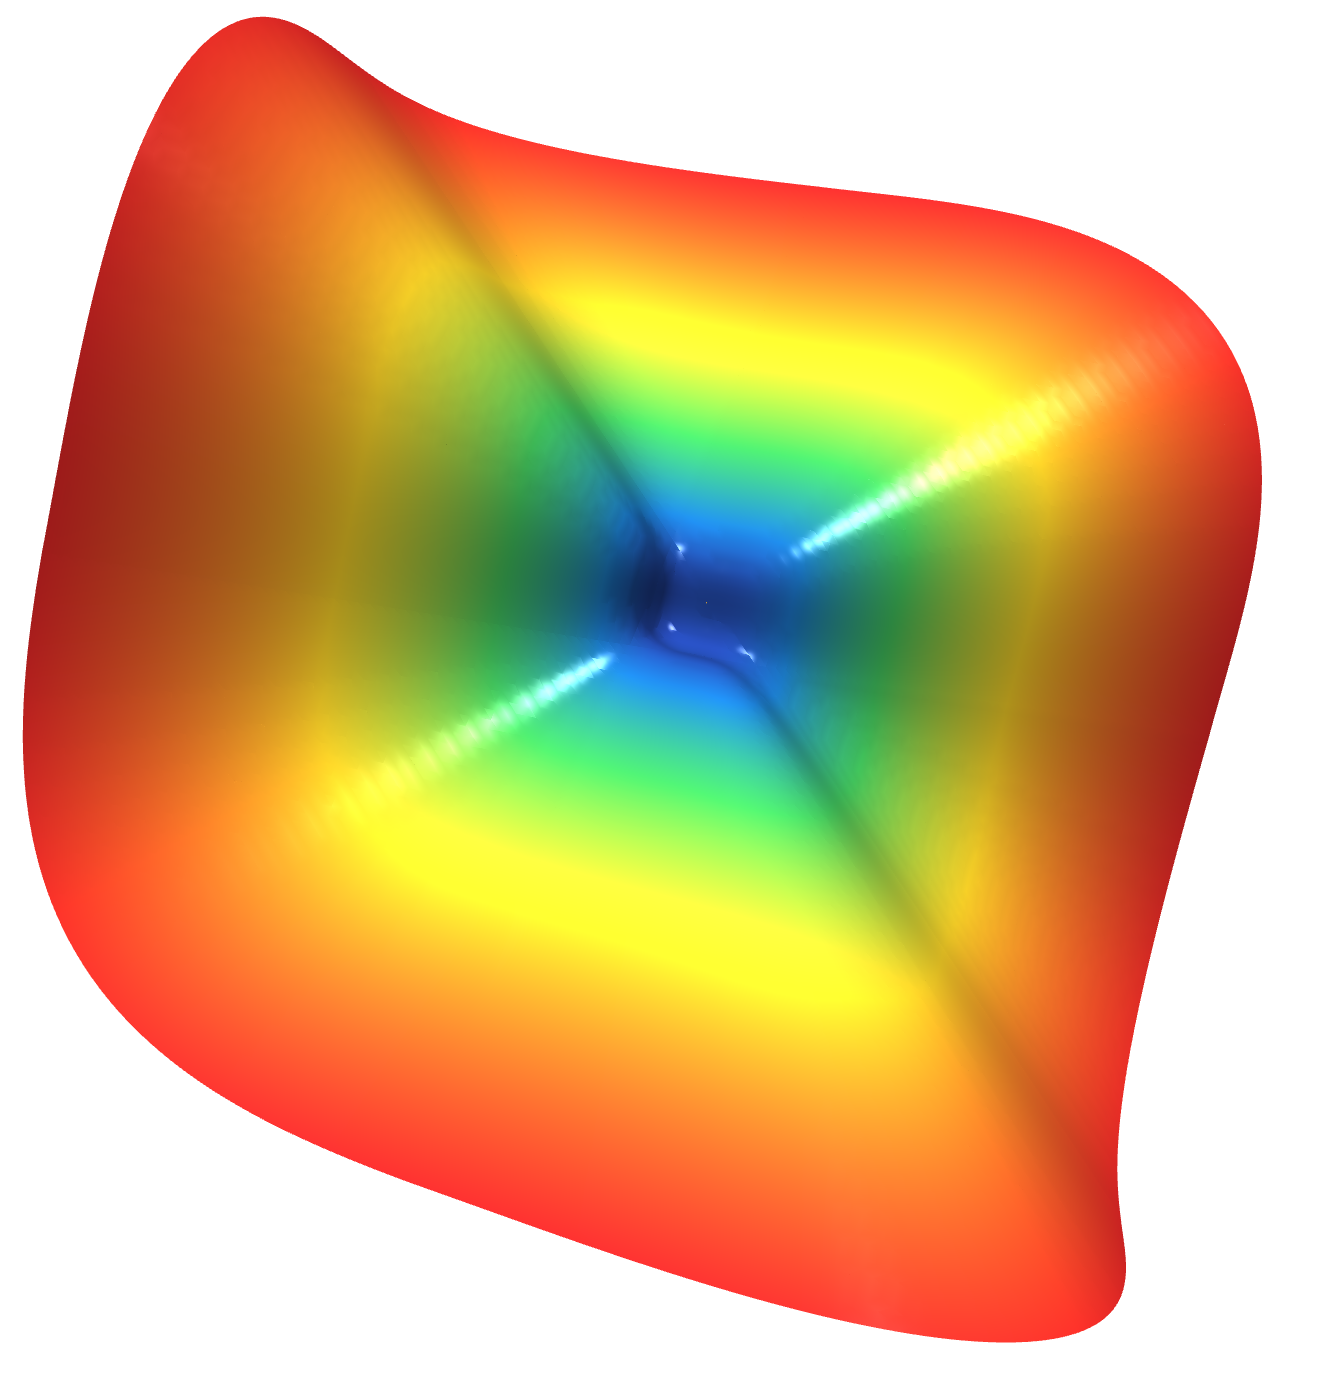
\includegraphics[width=0.7\linewidth]{pictures/ch4/G1_kneg.png}
        \caption{$k=-0.005$}
    \end{subfigure}
    \hfill
    \begin{subfigure}{0.31\textwidth}
        \centering
        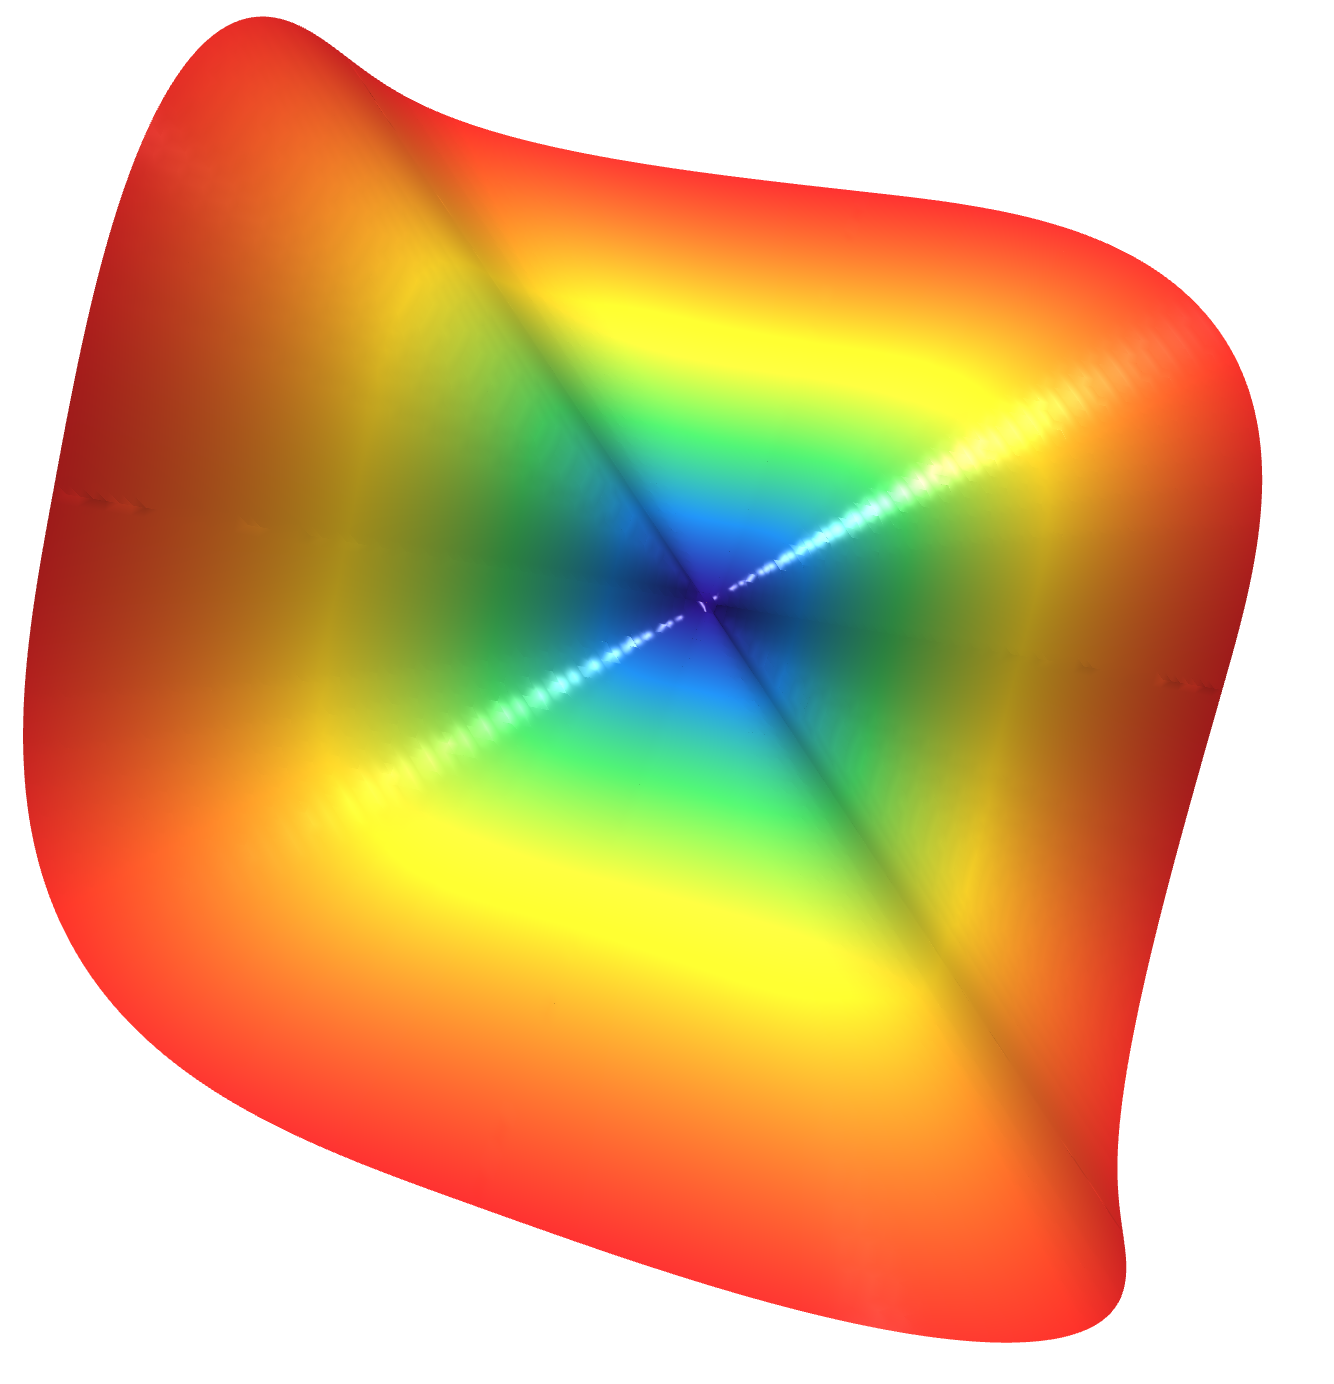
\includegraphics[width=0.7\linewidth]{pictures/ch4/G1_k0.png}
        \caption{$k=0$}
    \end{subfigure}
    \hfill
    \begin{subfigure}{0.31\textwidth}
        \centering
        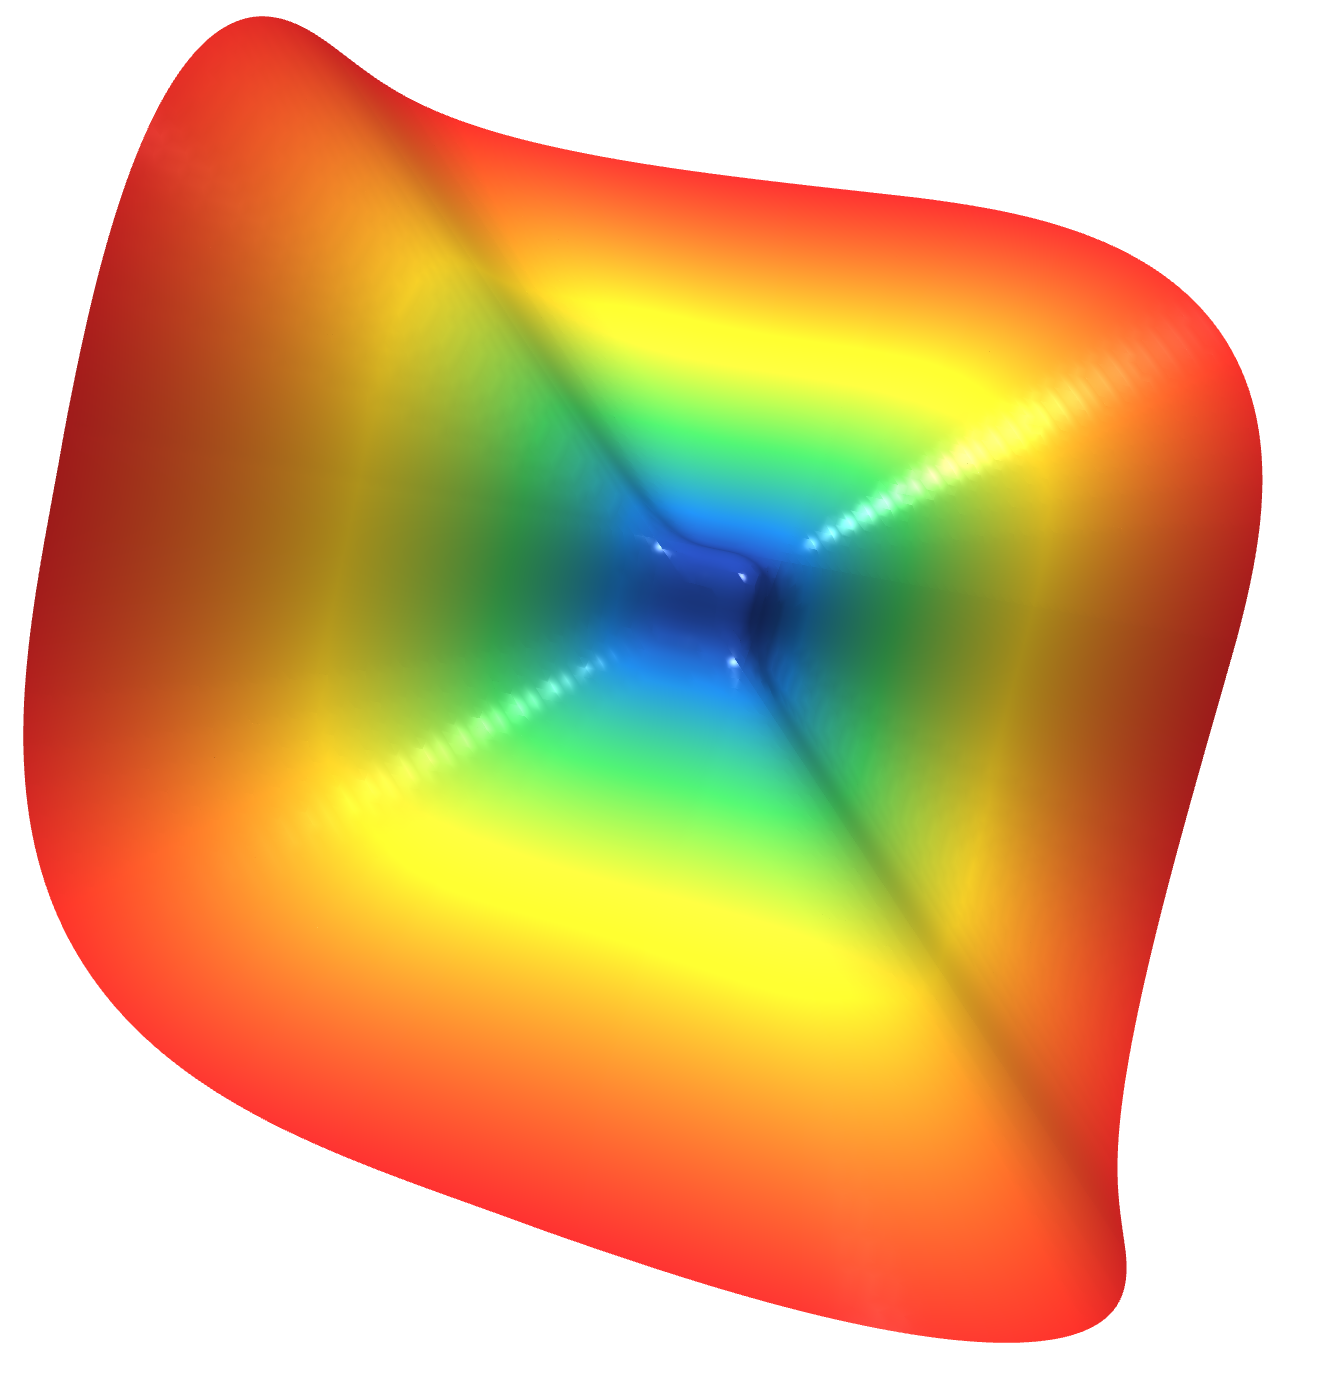
\includegraphics[width=0.7\linewidth]{pictures/ch4/G1_kpos.png}
        \caption{$k=+0.005$}
    \end{subfigure}
    \caption[Constant perturbation]{The constant perturbation moves the surface
    off the apex. For $k<0$ and $k>0$ the surface lies on opposite sides of the
    cone; in both cases it is regular.}
    \label{fig:constant-triptych}
\end{figure}

% -----------------------------------------------------------------------------
\section{Linear Perturbations}
\label{sec:linear-results}

\subsection{Coordinate perturbations}

For $G=x$, $y$ or $z$ the origin stays on the surface and becomes regular, with
$\nabla H_k(0)=k\nabla G(0)$. The measured minimum of $\|\nabla H_k\|$ on the
local mesh equals $|k|$ to six significant digits for every $k$, and the stationary-point
search finds the two points $(\pm\sqrt{-k/3},0,0)$ for $k<0$ (for $G=x$), which
lie off the zero level, as predicted by Example~\ref{ex:linear-cases}. The
distance from the origin to the mesh is zero for every $k$; it says nothing
about the deformation, which has to be measured by $d_R(k)$.

\begin{table}[!h]
\centering
\small
\begin{tabular}{c c c c}
\toprule
Cells per axis & $h$ & $\alpha$ for $k<0$ & $\alpha$ for $k>0$ \\
\midrule
$48$  & $0.016667$ & $0.505$ & $0.402$ \\
$96$  & $0.008333$ & $0.513$ & $0.472$ \\
$110$ & $0.007273$ & $0.510$ & $0.478$ \\
\midrule
predicted & & $0.5$ & $0.5$ \\
\bottomrule
\end{tabular}
\caption[Coordinate perturbation: rates]{Fitted exponent of the triangle-sampled
local Hausdorff distance for $F_++kx$, using all twelve values of $k$ on each
side. $F_-+kx$ gives the same values, and $F_-+kz$ the same values with the two
sides exchanged.}
\label{tab:coordinate-rates}
\end{table}

Table~\ref{tab:coordinate-rates} shows the measured rates. The negative side
agrees with the prediction $\alpha=1/2$ at every resolution. On the positive
side the estimate approaches $1/2$ under refinement but remains lower. The
reason is visible in the data: for $k>0$ the deformation is about $3.5$ times
smaller (its constant is $C\approx0.29$ instead of $C\approx1.0$), so the
measured values are closer to the discretisation error of the meshes. An error
that does not depend on $k$ adds to $C|k|^{1/2}$ and flattens the fitted slope;
it decreases with $h$, which is why the estimate improves from $0.40$ to $0.48$.
The asymmetry itself is geometric: for $k<0$ the cubic $x^3+kx$ has the
additional real roots $x=\pm\sqrt{-k}$, so the surface develops two extra
sheets near the $x$-axis, while for $k>0$ it does not.

\begin{figure}[!h]
\centering
\begin{tikzpicture}
\begin{axis}[
    width=0.62\textwidth, height=0.45\textwidth,
    xmode=log, ymode=log,
    xlabel={$|k|$}, ylabel={$d_R(k)$},
    legend pos=south east, legend cell align=left, legend style={font=\small},
    grid=major, grid style={gray!25}]
\addplot[only marks, mark=*, mark size=1.5pt, blue] coordinates {
(0.000833333,0.0288911) (0.00166667,0.0410596) (0.0025,0.0503086) (0.00333333,0.0589332)
(0.00416667,0.0657168) (0.005,0.072418) (0.00583333,0.0776703) (0.00666667,0.083606)
(0.0075,0.088605) (0.00833333,0.0932705) (0.00916667,0.0982818) (0.01,0.102538)};
\addlegendentry{$G=x$, $k<0$}
\addplot[only marks, mark=o, mark size=1.8pt, blue] coordinates {
(0.000833333,0.00918692) (0.00166667,0.0120469) (0.0025,0.0149821) (0.00333333,0.0169704)
(0.00416667,0.0190615) (0.005,0.0209543) (0.00583333,0.0226133) (0.00666667,0.024138)
(0.0075,0.0255514) (0.00833333,0.0269047) (0.00916667,0.0281542) (0.01,0.0294011)};
\addlegendentry{$G=x$, $k>0$}
\addplot[only marks, mark=square*, mark size=1.4pt, red] coordinates {
(0.000833333,0.0385637) (0.00166667,0.05569) (0.0025,0.0685128) (0.00333333,0.0789781)
(0.00416667,0.0883609) (0.005,0.0969538) (0.00583333,0.104904) (0.00666667,0.111947)
(0.0075,0.119016) (0.00833333,0.125453) (0.00916667,0.131732) (0.01,0.137562)};
\addlegendentry{$G=x+y$, $k<0$}
\addplot[only marks, mark=square, mark size=1.6pt, red] coordinates {
(0.000833333,0.0108923) (0.00166667,0.015338) (0.0025,0.0185843) (0.00333333,0.0215617)
(0.00416667,0.0237728) (0.005,0.0261346) (0.00583333,0.0282121) (0.00666667,0.030125)
(0.0075,0.0320583) (0.00833333,0.0338874) (0.00916667,0.0355084) (0.01,0.0369923)};
\addlegendentry{$G=x+y$, $k>0$}
\addplot[black, dashed, domain=0.0007:0.012, samples=10] {1.0*x^(1/2)};
\addlegendentry{slope $1/2$}
\addplot[black, dashed, domain=0.0007:0.012, samples=10, forget plot] {0.29*x^(1/2)};
\addplot[gray, densely dotted, domain=0.0007:0.012, samples=2] {0.0036};
\addlegendentry{$h/2$}
\end{axis}
\end{tikzpicture}
\caption[Linear perturbations: local Hausdorff distance]{Triangle-sampled local
Hausdorff distance for $F_++kG$ with $G=x$ and $G=x+y$, resolution $110$. All
four series are parallel to the reference lines of slope $1/2$. The dotted line
marks half of the grid spacing, below which distances are not resolved.}
\label{fig:linear-plot}
\end{figure}

\begin{figure}[!h]
    \centering
    \thesisimage{pictures/ch4/x_slices.png}{0.95\textwidth}{6cm}{Snapshot of $F_+ + kx$: three $z$-slices around $z=0$ (rows) for $k=-0.001,\ 0,\ +0.001$ (columns), the same $6\times6$ node window at the origin, isovalues printed at the nodes, resolution 110}
    \caption[Coordinate perturbation: slices]{Grid-aligned slices of
    $F_++kx$ near the origin. For $k=0$ the contour has a corner at the origin;
    for $k\neq0$ it passes through the origin smoothly, with a slope that
    depends on the sign of $k$.}
    \label{fig:x-slices}
\end{figure}

\subsection{Sums of coordinates and the balance condition}

The pairwise sums $x+y$, $x+z$ and $y+z$ are the first perturbations that
create singular points. For $F_+$ and $G=x+y$, Proposition~\ref{prop:linear}
predicts two cusps
\begin{equation}
\label{eq:pair-singularities}
q_\pm(k)=\Big(\pm\sqrt{-\tfrac k3},\ \mp\sqrt{-\tfrac k3},\ 0\Big),\qquad
\|q_\pm(k)\|=\sqrt{\tfrac{2|k|}{3}},\qquad k<0,
\end{equation}
and none for $k>0$. The stationary-point search finds exactly these two points
for each of the twelve negative values of $k$, at all three resolutions; at
$k=-0.01$ they are $(\pm0.0577350,\mp0.0577350,0)$, with $H_k$ of order
$10^{-22}$ at both. Their Hessian has rank two, which confirms the cusp type.
The two other stationary points $\pm(\sqrt{-k/3},\sqrt{-k/3},0)$, with equal
signs, lie off the zero level. The origin itself is regular, with
$\|\nabla H_k(0)\|=\sqrt2\,|k|$, which is again the measured minimum gradient
for $k>0$.

\begin{figure}[!h]
\centering
\begin{tikzpicture}
\begin{axis}[
    width=0.62\textwidth, height=0.42\textwidth,
    xmode=log, ymode=log,
    xlabel={$|k|$, $k<0$}, ylabel={$\|q(k)\|$},
    legend pos=north west, legend cell align=left, legend style={font=\small},
    grid=major, grid style={gray!25}]
\addplot[only marks, mark=*, mark size=1.5pt, red] coordinates {
(0.000833333,0.0235702) (0.00166667,0.0333333) (0.0025,0.0408248) (0.00333333,0.0471405)
(0.00416667,0.0527046) (0.005,0.057735) (0.00583333,0.062361) (0.00666667,0.0666667)
(0.0075,0.0707107) (0.00833333,0.0745356) (0.00916667,0.0781736) (0.01,0.0816497)};
\addlegendentry{$G=x+y$ (cusps)}
\addplot[red, domain=0.0007:0.012, samples=10] {sqrt(2*x/3)};
\addlegendentry{$\sqrt{2|k|/3}$}
\addplot[only marks, mark=square*, mark size=1.4pt, teal] coordinates {
(0.000833333,0.0315674) (0.00166667,0.044643) (0.0025,0.0546763) (0.00333333,0.0631348)
(0.00416667,0.0705868) (0.005,0.077324) (0.00583333,0.0835195) (0.00666667,0.0892861)
(0.0075,0.0947022) (0.00833333,0.0998249) (0.00916667,0.104697) (0.01,0.109353)};
\addlegendentry{$G=x+y+2^{2/3}z$ (nodes)}
\addplot[teal, domain=0.0007:0.012, samples=10] {sqrt(x/3)*sqrt(2+1.5874010519681994)};
\addlegendentry{equation~\eqref{eq:singular-distance}}
\end{axis}
\end{tikzpicture}
\caption[Singular points converging to the origin]{Distance of the singular
points found numerically from the origin, for $F_++kG$ and $k<0$, compared
with the exact formula~\eqref{eq:singular-distance}. Both families converge
with rate $\gamma=1/2$.}
\label{fig:singular-plot}
\end{figure}

\begin{figure}[!h]
    \centering
    \begin{subfigure}{0.47\textwidth}
        \centering
        \thesisimage{pictures/ch4/xy_3d.png}{\textwidth}{5cm}{3D view of $F_+ + k(x+y)$, $k=-0.01$, the two cusps marked}
        \caption{3D view, $k=-0.01$}
    \end{subfigure}
    \hfill
    \begin{subfigure}{0.47\textwidth}
        \centering
        \thesisimage{pictures/ch4/xy_slice_z0.png}{\textwidth}{5cm}{Slice $z=0$ (the plane of the cusps), $k=-0.01$, node window around the origin}
        \caption{slice $z=0$}
    \end{subfigure}
    \caption[Pairwise perturbation]{$F_++k(x+y)$ for $k<0$: the cone is opened
    at the origin, and two cusps appear on the line $x=-y$ in the plane
    $z=0$.}
    \label{fig:pair-singular}
\end{figure}

The remaining linear perturbations confirm the balance condition. For $F_+$,
$x+z$ and $y+z$ behave like $x+y$; $x+y+z$, $2x+4y+6z$, $9x+y+3z$, $x+2y+3z$
and $2x+4y+z$ produce stationary points for $k<0$ but no singular points. For
$F_-$, the perturbations $x+z$, $y+z$, $x+y+z$ and $2x+4y+6z$ produce no real
stationary points at all, while $x+y$ produces the same two cusps as for $F_+$.
The decisive test is the perturbation $G=x+y+2^{2/3}z$, which was constructed
from~\eqref{eq:balance} before it was computed: the theory predicts two ordinary
double points with all three coordinates nonzero, and the search finds exactly
two, for example $(-0.057735,-0.057735,0.072742)$ at $k=-0.01$, with full-rank
Hessian and the distances shown in Figure~\ref{fig:singular-plot}. For $F_-$ the
same holds for $x+y-2^{2/3}z$.

\begin{figure}[!h]
    \centering
    \thesisimage{pictures/ch4/balanced_3d.png}{0.6\textwidth}{5cm}{3D view of $F_+ + k(x+y+1.5874z)$, $k=-0.01$, the two ordinary double points marked}
    \caption[Balanced perturbation]{The balanced perturbation
    $G=x+y+2^{2/3}z$ creates two ordinary double points (quadratic cones) off
    the coordinate planes.}
    \label{fig:balanced}
\end{figure}

\subsection{Mixed linear--quadratic perturbations}

The perturbations $x^2+x$, $x^2+y$ and $x^2+z$ have degree two but order one.
The origin stays on the surface as a regular point, the measured minimum
gradient is again $|k|$, and no singular points are found, as expected from the
model surface, which depends only on the linear part. Their rates agree with
the linear perturbations: $0.54/0.44$ for $x^2+x$, $0.53/0.45$ for $x^2+y$ and
$x^2+z$ (negative and positive side, logarithmic sampling, resolution 110).
The order, not the degree, determines the scale.

% -----------------------------------------------------------------------------
\section{Quadratic Perturbations}
\label{sec:quadratic-results}

For $G=x^2$, $y^2$ or $z^2$ the origin stays singular for every $k$. By
equation~\eqref{eq:translation}, $F_\sigma+kx^2$ is, up to terms of order $k^2$,
the cone translated by $k/3$ along the $x$-axis. The second-order terms split
the translated apex into two $D_4$ points, the origin and $(-2k/3,0,0)$,
symmetric about the translated apex at $-k/3$. Only the origin lies on the
zero level; at the other point $H_k=4k^3/27$. The search finds precisely these
two stationary points, with Hessian rank one at both; at $k=-0.01$ the second
one is $(0.00667,0,0)$.

Since the deformation is a translation by about $|k|/3$, the local Hausdorff
distance is linear in $|k|$, about $0.0058$ at $|k|=0.01$. This is less than one
grid cell, so the range $|k|\le0.01$ cannot measure a rate
(Section~\ref{sec:voxel-consequences}). With $|k|$ up to $0.3$ the fitted
exponents are $1.16$ ($k<0$) and $1.19$ ($k>0$), close to the predicted
$\alpha=1$; the slight excess comes from the $k^2$ terms in~\eqref{eq:translation},
which are no longer negligible at the upper end of this range.

The perturbation $x^2+y^2+z^2$ makes the origin an ordinary double point,
because $\operatorname{Hess}H_k(0)=2k\,I$ is nonsingular. Its seven other
stationary points, with coordinates in $\{0,-2k/3\}$, satisfy
$H_k=\tfrac{4k^3}{27}n\neq0$, where $n$ is the number of nonzero coordinates,
and all eight are found by the search. The perturbation $x^2+y^2-z^2$ is
richer. Its eight stationary points have coordinates in $\{0,-2k/3\}$ for $x,y$
and in $\{0,2k/3\}$ for $z$, and
\[
H_k=\frac{4k^3}{27}\,(n_{xy}-n_z),
\]
where $n_{xy}\in\{0,1,2\}$ counts the nonzero coordinates among $x,y$ and
$n_z\in\{0,1\}$ the nonzero $z$-coordinate. The zero level is reached for
$n_{xy}=n_z$: at the origin and at the two points $(-2k/3,0,2k/3)$ and
$(0,-2k/3,2k/3)$. All eight are ordinary double points, which accounts for the
Milnor number $8$ (Table~\ref{tab:milnor-conservation}). The two singular points
away from the origin converge linearly, $\|q(k)\|=\tfrac{2\sqrt2}{3}|k|$, and the
search finds them with measured rate $\gamma=1.00$.

\begin{figure}[!h]
    \centering
    \begin{subfigure}{0.47\textwidth}
        \centering
        \thesisimage{pictures/ch4/x2_k0.png}{\textwidth}{5cm}{$F_+$, $k=0$, 3D view}
        \caption{$k=0$}
    \end{subfigure}
    \hfill
    \begin{subfigure}{0.47\textwidth}
        \centering
        \thesisimage{pictures/ch4/x2_k03.png}{\textwidth}{5cm}{$F_+ + kx^2$, $k=0.3$, same view; the apex is moved along $x$}
        \caption{$k=0.3$}
    \end{subfigure}
    \caption[Quadratic perturbation]{The perturbation $x^2$ acts, to first
    order, as a translation of the cone by $k/3$ along the $x$-axis; the
    singular point stays at the origin and becomes a $D_4$ point.}
    \label{fig:quadratic}
\end{figure}

\begin{figure}[!h]
    \centering
    \thesisimage{pictures/ch4/x2y2mz2.png}{0.6\textwidth}{5cm}{3D view of $F_+ + k(x^2+y^2-z^2)$, $k=-0.1$, domain $\pm0.4$; the three singular points (origin, $(-2k/3,0,2k/3)$, $(0,-2k/3,2k/3)$) marked}
    \caption[Quadratic perturbation with three singular points]{$F_++k(x^2+y^2-z^2)$:
    the origin and two further ordinary double points, which converge to the
    origin linearly in $k$.}
    \label{fig:three-singular}
\end{figure}

% -----------------------------------------------------------------------------
\section{Cubic Perturbations}
\label{sec:cubic-results}

For $G=x^3$, equation~\eqref{eq:stretch} shows that $S_k$ is the cone $S_0$
stretched by the factor $(1+k)^{-1/3}$ along the $x$-axis: the singularity is
unchanged ($\tilde E_6$, $\mu=8$), and only the opening of the cone changes. The
same holds for $y^3$ and $z^3$, and for $F_-$. A point at distance $r$ from the
origin moves by at most $|1-(1+k)^{-1/3}|\,r\approx|k|r/3$, so
$d_R(k)\le|k|R/3$. At $|k|=0.01$ this bound is $0.00055$, and the measured value
is $0.00029$, about four percent of a grid cell. Even at $|k|=0.3$ fewer than
three values exceed half a grid cell, and no rate can be fitted. The cubic
perturbations are therefore classified as \emph{below resolution}, not as
non-converging; the theory gives $\alpha=1$.

The perturbation $G=F$ gives $H_k=(1+k)F$, whose zero set is $S_0$ for every
$k\neq-1$. The measured Hausdorff distance is zero, which serves as a check of
the measurement.

% -----------------------------------------------------------------------------
\section{Summary of the Classification}
\label{sec:classification-summary}

Table~\ref{tab:classification} summarises all experiments for $F_+$ with
logarithmic sampling at resolution $110$. The results for $F_-$ coincide after
the reflection~\eqref{eq:reflection}; the differences are listed below the table.

\begin{table}[!h]
\centering
\footnotesize
\setlength{\tabcolsep}{4pt}
\begin{tabular}{l c l c c l}
\toprule
$G$ & $m$ & origin & $\alpha$ pred. & $\alpha$ meas. ($k<0$/$k>0$) & singular points ($k<0$ / $k>0$) \\
\midrule
$1$                        & 0 & leaves  & $1/3$ & $0.34$ / $0.34$ & none / none \\
$x$, $y$, $z$              & 1 & regular & $1/2$ & $0.53$ / $0.43$ & none / none \\
$x+y$, $x+z$, $y+z$        & 1 & regular & $1/2$ & $0.51$ / $0.48$ & 2 cusps, $\gamma=0.50$ / none \\
$x+y+z$                    & 1 & regular & $1/2$ & $0.53$ / $0.44$ & none / none \\
$2x+4y+6z$                 & 1 & regular & $1/2$ & $0.52$ / $0.49$ & none / none \\
$9x+y+3z$                  & 1 & regular & $1/2$ & $0.52$ / $0.50$ & none / none \\
$x+2y+3z$                  & 1 & regular & $1/2$ & $0.51$ / $0.48$ & none / none \\
$2x+4y+z$                  & 1 & regular & $1/2$ & $0.50$ / $0.49$ & none / none \\
$x+y+2^{2/3}z$             & 1 & regular & $1/2$ & $0.51$ / $0.46$ & 2 nodes, $\gamma=0.50$ / none \\
$x^2+x$                    & 1 & regular & $1/2$ & $0.54$ / $0.44$ & none / none \\
$x^2+y$, $x^2+z$           & 1 & regular & $1/2$ & $0.53$ / $0.45$ & none / none \\
$x^2$, $y^2$, $z^2$        & 2 & singular ($D_4$) & $1$ & $1.16$ / $1.19$ & origin / origin \\
$x^2+y^2+z^2$              & 2 & singular ($A_1$) & $1$ & $1.16$ / $1.16$ & origin / origin \\
$x^2+y^2-z^2$              & 2 & singular ($A_1$) & $1$ & $1.12$ / $1.05$ & origin + 2 nodes, $\gamma=1$ (both) \\
$x^3$, $y^3$, $z^3$        & 3 & singular ($\tilde E_6$) & $1$ & below resolution & origin / origin \\
$F$                        & 3 & singular ($\tilde E_6$) & --- & identical & origin / origin \\
\bottomrule
\end{tabular}
\caption[Classification of all experiments]{Classification of the
perturbations of $F_+$ (logarithmic sampling, resolution $110$, $|k|\le0.01$ for
$m\le1$ and $|k|\le0.3$ for $m\ge2$). ``Origin'' describes the original
singular point for $k\neq0$; $\alpha$ is the rate of the local Hausdorff
distance and $\gamma$ the rate at which new singular points approach the
origin.}
\label{tab:classification}
\end{table}

For $F_-$ the results agree with Table~\ref{tab:classification} except for the
following entries: $z$ and $x^2+z$ exchange their two measured exponents;
$x+z$, $y+z$, $x+y+z$ and $2x+4y+6z$ create no singular points and give rates
$0.50$--$0.52$ on both sides; and the balanced perturbation is
$x+y-2^{2/3}z$.

% -----------------------------------------------------------------------------
\section{Self-Similarity of the Inner Region}
\label{sec:self-similarity}

Proposition~\ref{prop:scaling} predicts more than a rate: near the origin, $S_k$
is a copy of the fixed model surface $M_\sigma$ scaled by $\lambda(k)$. For
$F_++kx$ this holds exactly, not only asymptotically. Since $F_+$ is homogeneous
of degree three and $x$ of degree one,
\[
H_k(\lambda u)=\lambda^3\big(F_+(u)+\sigma u_1\big)\qquad\text{for }\lambda=\sqrt{|k|},
\]
so $S_k=\lambda(k)M_\sigma$ for every $k$ of a fixed sign. This can be observed
directly: for $k=0.01$, $0.04$ and $0.16$ the scale $\lambda$ doubles from one
value to the next. If the domain is scaled with it, here to the half-extent
$4\lambda$, and the resolution is kept fixed, the three extracted surfaces must
be identical up to the factor $\lambda$. Figure~\ref{fig:self-similar} shows the
same grid window at the three parameter values.

\begin{figure}[!h]
    \centering
    \begin{subfigure}{0.31\textwidth}
        \centering
        \thesisimage{pictures/ch4/selfsimilar_a.png}{\textwidth}{4cm}{$F_+ + kx$, $k=0.01$, half-extent $0.4$, slice $z=0$}
        \caption{$k=0.01$}
    \end{subfigure}
    \hfill
    \begin{subfigure}{0.31\textwidth}
        \centering
        \thesisimage{pictures/ch4/selfsimilar_b.png}{\textwidth}{4cm}{$k=0.04$, half-extent $0.8$, same slice and window}
        \caption{$k=0.04$}
    \end{subfigure}
    \hfill
    \begin{subfigure}{0.31\textwidth}
        \centering
        \thesisimage{pictures/ch4/selfsimilar_c.png}{\textwidth}{4cm}{$k=0.16$, half-extent $1.6$, same slice and window}
        \caption{$k=0.16$}
    \end{subfigure}
    \caption[Self-similarity]{Self-similarity of the inner region for
    $F_++kx$. The domain is scaled with $\lambda(k)=\sqrt{|k|}$ and the grid
    resolution is fixed; the contours coincide, and the isovalues scale by
    $\lambda^3$.}
    \label{fig:self-similar}
\end{figure}

% -----------------------------------------------------------------------------
\section{Resolution and Numerical Reliability}
\label{sec:resolution-study}

Table~\ref{tab:resolution} compares the three grids for $F_-+kx$. The number of
triangles grows with $h^{-2}$, as expected for a surface, and the largest field
residual $|H_k|$ at mesh vertices near the origin decreases with $h$. The build
times were measured with the families processed in parallel on a ten-core
computer and are given only for comparison between the grids.

\begin{table}[!h]
\centering
\small
\begin{tabular}{c c c c c}
\toprule
Cells per axis & $h$ & Median triangles & Median build time & Largest local residual \\
\midrule
$48$  & $0.016667$ & $12\,932$ & $3.5$ ms  & $2.60\cdot10^{-5}$ \\
$96$  & $0.008333$ & $51\,960$ & $30.4$ ms & $1.19\cdot10^{-5}$ \\
$110$ & $0.007273$ & $68\,236$ & $58.2$ ms & $5.34\cdot10^{-6}$ \\
\bottomrule
\end{tabular}
\caption[Resolution comparison]{Cost and accuracy of the three grids for
$F_-+kx$ over the $25$ values of $k$.}
\label{tab:resolution}
\end{table}

The finer grids improve every measured quantity: the constant of
Proposition~\ref{prop:constant-distance} is reproduced to $6\cdot10^{-5}$, and
the positive-side rate of the coordinate perturbation moves towards $1/2$. The
resolution required, however, depends on the order of the perturbation rather
than on the surface. At the smallest tested $|k|=8.3\cdot10^{-4}$ the linear
scale $\sqrt{|k|}\approx0.029$ spans four cells of the finest grid, whereas the
quadratic deformation $|k|/3$ spans only $0.04$ of a cell, and the cubic one
less still. Uniform refinement is an expensive remedy, since the number of
triangles grows quadratically with $1/h$; locally adaptive refinement near the
singular point, or the analytic results of
Chapter~\ref{ch:perturbation-theory}, are the appropriate tools for these
small deformations (Figure~\ref{fig:resolution-images}).

\begin{figure}[!h]
    \centering
    \begin{subfigure}{0.47\textwidth}
        \centering
        \thesisimage{pictures/ch4/resolution_48.png}{\textwidth}{5cm}{$F_+ + k(x+y)$, $k=-0.0025$, slice $z=0$, resolution 48}
        \caption{48 cells per axis}
    \end{subfigure}
    \hfill
    \begin{subfigure}{0.47\textwidth}
        \centering
        \thesisimage{pictures/ch4/resolution_110.png}{\textwidth}{5cm}{same family, $k$ and slice, resolution 110}
        \caption{110 cells per axis}
    \end{subfigure}
    \caption[Effect of the resolution]{The two cusps of $F_++k(x+y)$ at
    $k=-0.0025$, at distance $0.041$ from the origin, are separated by $0.082$, about
    five cells of the coarse grid and eleven cells of the fine grid.}
    \label{fig:resolution-images}
\end{figure}

% -----------------------------------------------------------------------------
\section{Limitations}
\label{sec:limitations}

The numerical results support the analysis, but several measured quantities
have to be read with care.
\begin{itemize}
    \item The distance from the origin to the mesh is zero whenever $G(0)=0$.
          It measures whether the origin is on the surface, not how much the
          surface changes.
    \item The minimum gradient is taken over mesh vertices. It approximates the
          minimum over the continuous surface from above, and a singular point
          between vertices can have a small positive sampled value. Where the
          origin stays singular, the sampled minimum is dominated by the grid
          and its dependence on $k$ is not meaningful.
    \item The stationary-point search is local and numerical. At degenerate
          points such as the cusps, Newton's method converges only linearly in
          the degenerate direction, and the same point can be returned twice,
          about $10^{-8}$ apart; such duplicates are merged. A search that finds
          no singular point is evidence, not proof; the counts in this chapter
          are confirmed by the exact solutions of
          Section~\ref{sec:linear-perturbation}.
    \item The sampled Hausdorff distance approximates
          Definition~\ref{def:local-hausdorff} from below, and its accuracy is
          limited by the mesh, of the order of $h$. Rates are therefore fitted
          only inside the window $h/2\le d\le0.6R$.
    \item A high $R^2$ shows that the data lie on a straight line in logarithmic
          coordinates over the sampled range. It does not show that the
          fitted exponent equals the theoretical one, nor that the law holds
          outside that range.
    \item Where the real lines of the cone pass through grid nodes, the
          tie-break of the extractor cannot always separate the edge
          intersections. In the quadratic families, where these nodes lie on
          the perturbed surface as well, $8645$ degenerate triangles were
          discarded in total, about twenty per mesh of some $68\,000$
          triangles. The other families contain none.
\end{itemize}

% -----------------------------------------------------------------------------
\section{Conclusions}
\label{sec:experimental-conclusions}

The experiments answer the questions posed at the beginning of
Chapter~\ref{ch:perturbation-theory} for the reference cones $F_\pm$.
\begin{enumerate}
    \item \textbf{The surfaces always converge.} By the sign-change criterion,
          $S_k$ converges to $S_0$ from both sides for every perturbation; no
          experiment contradicts this.
    \item \textbf{The order of $G$ fixes the rate.} The local Hausdorff distance
          decreases like $|k|^{1/(3-m)}$: $|k|^{1/3}$ for a constant,
          $|k|^{1/2}$ for perturbations of order one, including $x^2+x$, and
          $|k|$ for orders two and three. The measured exponents agree with
          these predictions within the accuracy of the grid; for the constant
          perturbation the exact distance $|k|^{1/3}$ is reproduced to
          $6\cdot10^{-5}$.
    \item \textbf{The direction of $G$ decides the singular points.} Constant
          and single-coordinate perturbations remove the singularity. Linear
          perturbations create singular points exactly when the balance
          condition~\eqref{eq:balance} holds: cusps if one coefficient
          vanishes, ordinary double points if none does, in every case
          converging to the origin like $|k|^{1/2}$. Perturbations of order two
          keep the origin singular with a simpler type ($D_4$ or $A_1$) and can
          add further singular points converging linearly. Perturbations that
          are coordinate changes, such as $x^3$ and $F$ itself, leave the
          singularity unchanged.
    \item \textbf{At most eight singular points can appear}, because the Milnor
          number of the reference singularity is eight; the experiments show
          the redistribution of this number in every case examined.
    \item \textbf{What the grid can see is set by $\lambda(k)$.} Effects of
          order zero and one are resolved on the tested grids; effects of order
          two and three are below the grid spacing for $|k|\le0.01$ and require
          larger parameters, adaptive refinement, or analytic treatment.
\end{enumerate}
These results identify the order of the perturbation at the singular point,
its essential direction in the sense of
Section~\ref{sec:perturbation-vector}, and the ratio $\lambda(k)/h$ as the three
quantities that determine whether a voxel method represents the neighbourhood
of the singularity faithfully.

\newpage

\bibliographystyle{alpha}
\bibliography{bibliography}

\end{document}
